\chapter{Image Process} \label{chapter:model}
The Image Process algorithms and Eulerian Color Magnification used are the main part of the software. The aim of image enhancement is to improve the interpretability or perception of information in images for human viewers.
  
\section{Overview}
For the skin indentation, reactive hyperameia was induced in the arms of different individuals. The arms were imaged and videoed. The Image Processing Algorithms are including brightness and contrast adjustment, histogram (RGB Histogram, Histogram Equalization, Contrast Limited Adaptive Equalizaiton) , filter (median filter, gaussian filter, Bilateral filter), and pressure ulcers area detection. The videos were processed through eularian colour magnification. 
    
\section{Brightness and Contrast Adjustments}
An image have the proper brightness and contrast for easier viewing. Brightness refers to the lightness or darkness of the image. Contrast is the difference in brightness between objects or regions.\\

In opencv, two used point processes are multiplication and addition with a contrast:
\begin{displaymath}
g(x) = \alpha f(x) + \beta 
\end{displaymath}
The parameters $\alpha$ $\textgreater$ 0 and $\beta$ are called control contrast and brightness respectively. And f(x) is the source image pixels and g(x) is the output image pixels. For each pixel in the image, using the syntax: 
\begin{displaymath}
image.at<Vec3b>(y,x)[c] 
\end{displaymath}
where y is the row, x is the column and c is R, G or B (0, 1 or 2). Figure 5.1 compares the original image and image after brightness and contrast adjustment. As showed, the image on the right side is brighter as compared to the image on the left.
\begin{figure}[!h]
\centering
\begin{subfigure}{.5\textwidth}
  \centering
  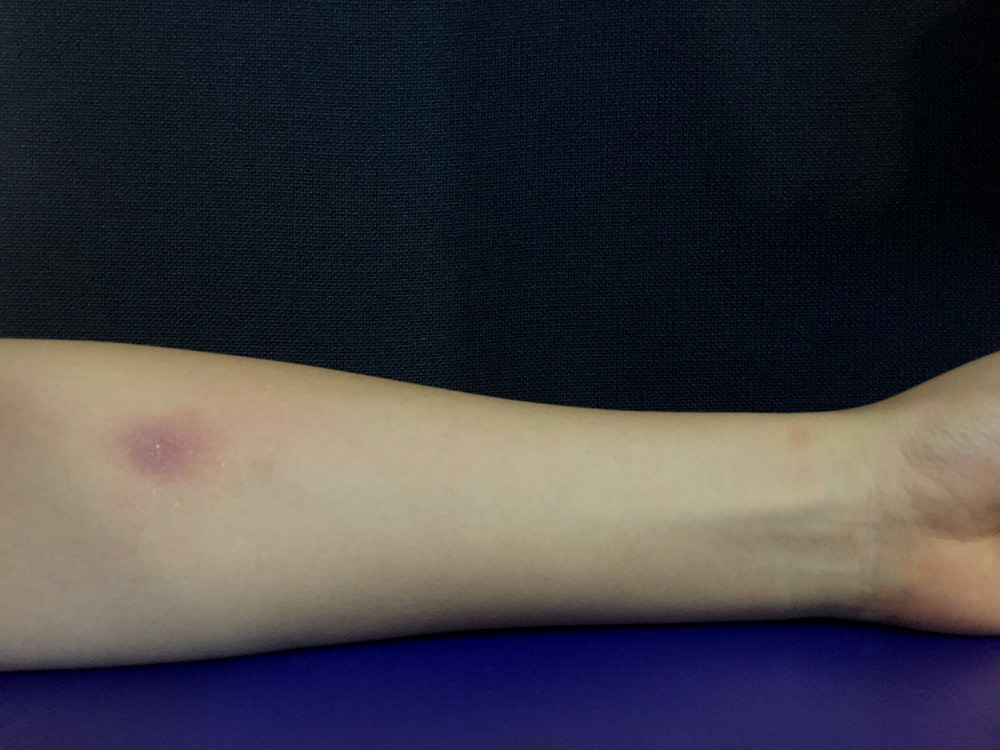
\includegraphics[scale=0.23]{img/original}
  \caption{Original Image}
  \label{fig:sub1}
\end{subfigure}%
\begin{subfigure}{.5\textwidth}
  \centering
  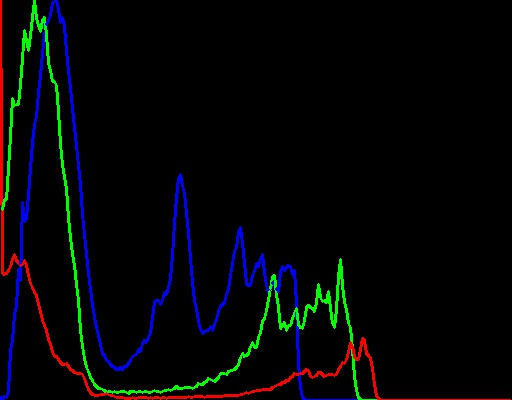
\includegraphics[scale=0.43]{img/image}
  \caption{RGB Histogram of Original Image}
  \label{fig:sub2}
\end{subfigure}
\begin{subfigure}{.5\textwidth}
  \centering
  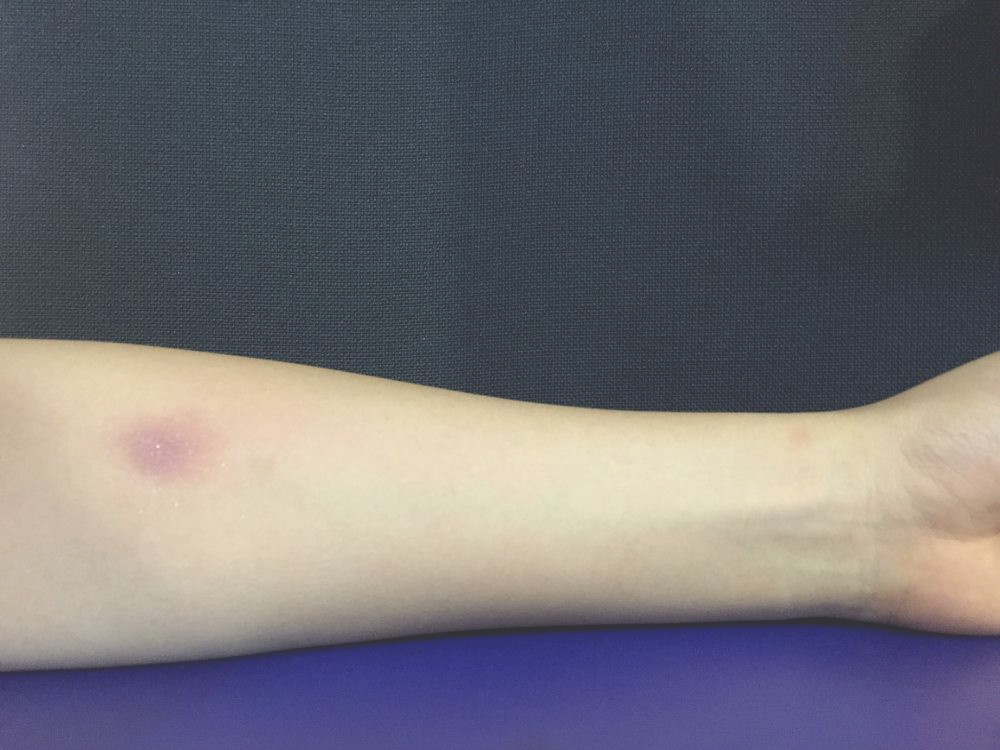
\includegraphics[scale=0.23]{img/brightresult}
  \caption{Image After Brightness and Contrast Adjustment}
  \label{fig:sub2}
\end{subfigure}%
\begin{subfigure}{.5\textwidth}
  \centering
  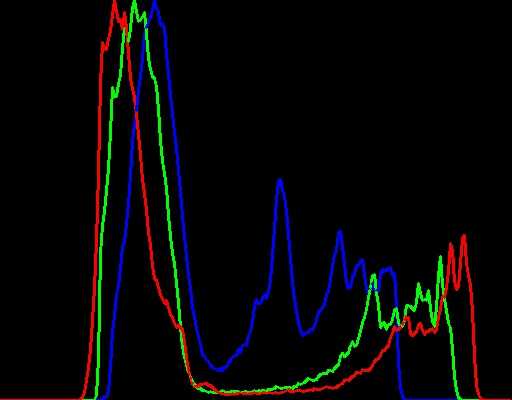
\includegraphics[scale=0.43]{img/imagergb}
  \caption{RGB Histogram of Result Image}
  \label{fig:sub2}
\end{subfigure}
\caption{Image After Brightness and Contrast Adjustment}
\label{fig:test}
\end{figure}

\newpage
For brightness, it is necessary to distinguish between true brightness and gamma. Increasing Gamma makes images look brighter, but it is non-linear, therefore it only increases brightness of the shadows and mid-tones in images without affecting the highlights. While traditional brightness brightens the entire image from the shadows to the highlights equally. Figure 5.2 presents the affect of adding and reducing brightness.
\begin{figure}[!h]
\centering
\begin{subfigure}{.35\textwidth}
  \centering
  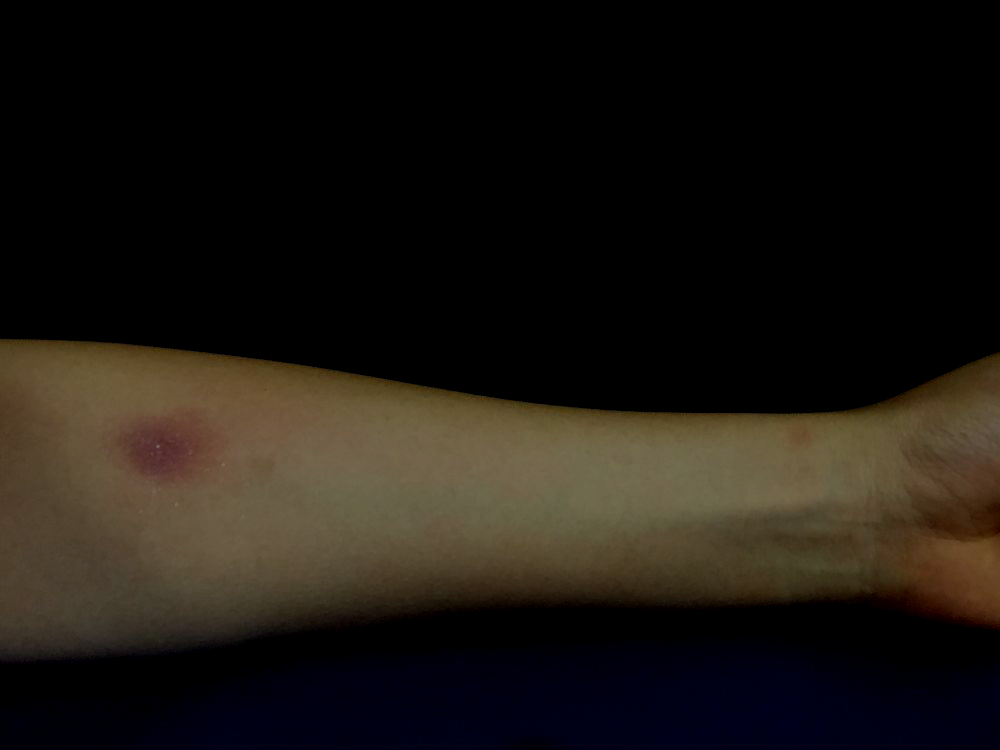
\includegraphics[scale=0.14]{img/bright1}
  \caption{Reduce Brightness}
  \label{fig:sub1}
\end{subfigure}%
\begin{subfigure}{.3\textwidth}
  \centering
  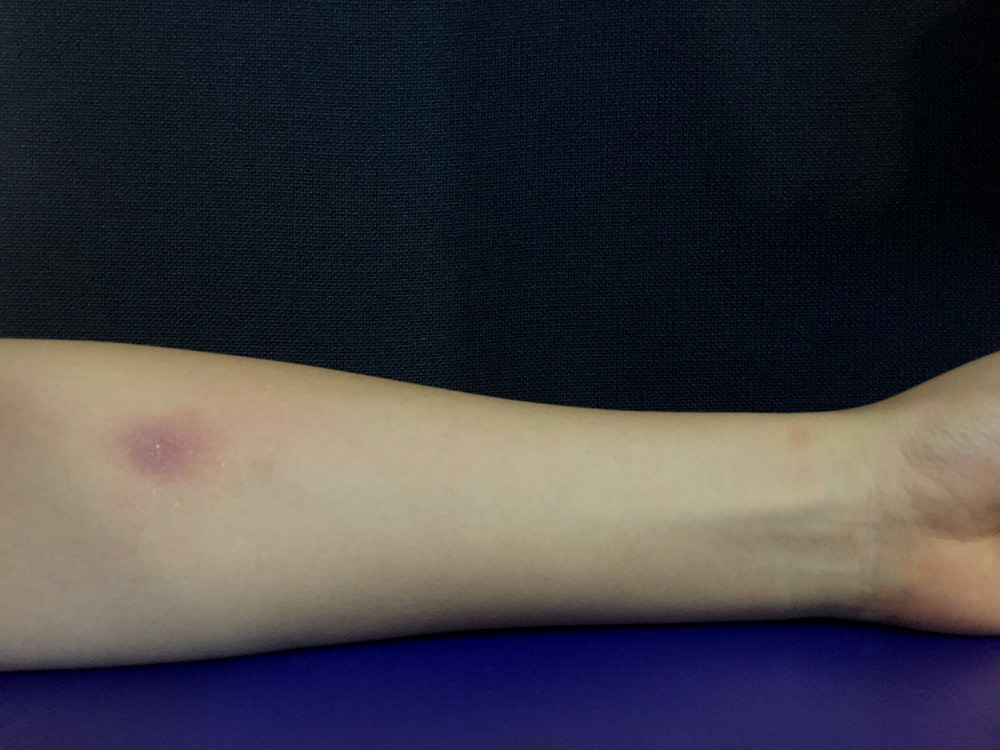
\includegraphics[scale=0.14]{img/original}
  \caption{Original Image}
  \label{fig:sub2}
\end{subfigure}
\begin{subfigure}{.3\textwidth}
  \centering
  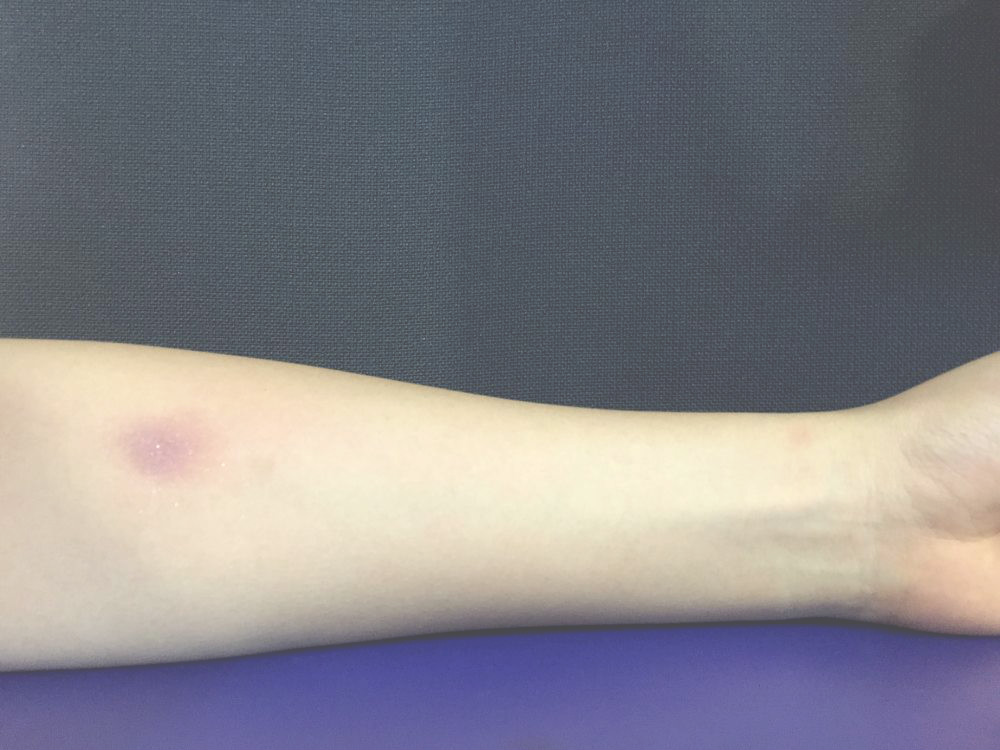
\includegraphics[scale=0.14]{img/bright2}
  \caption{Add Brightness}
  \label{fig:sub2}
\end{subfigure}
\caption{Reduce and Add Brightness of the Image}
\label{fig:test}
\end{figure}

If adding even more brightness, it may have clipped the white spokes in the wheel which would have affected contrast, what may be worse, the shadows will catch up to the highlights because they are as bright as they can get. The same effect can be seen if reducing brightness to the point that the shadows had nowhere else to go and the highlights catch up to the shadows. It depends on how close the shadows and highlights of the image are to the endpoints. When increasing brightness, the image loses some contrast on the brightest details while the rest of the image has the same contrast as before.\\

For contrast, it is the separation between the darkest and brightest areas of the image, which makes shadows darker and highlights brighter. Decreasing contrast will bring the shadows up and the highlights down to make them closer to each other. Figure 5.3 presents the affect of adding and reducing contrast. As Figure 5.3 shows, adding contrast make the hand gets brighter while the background gets darker, which cause the image to look more defined. 
\begin{figure}[!h]
\centering
\begin{subfigure}{.35\textwidth}
  \centering
  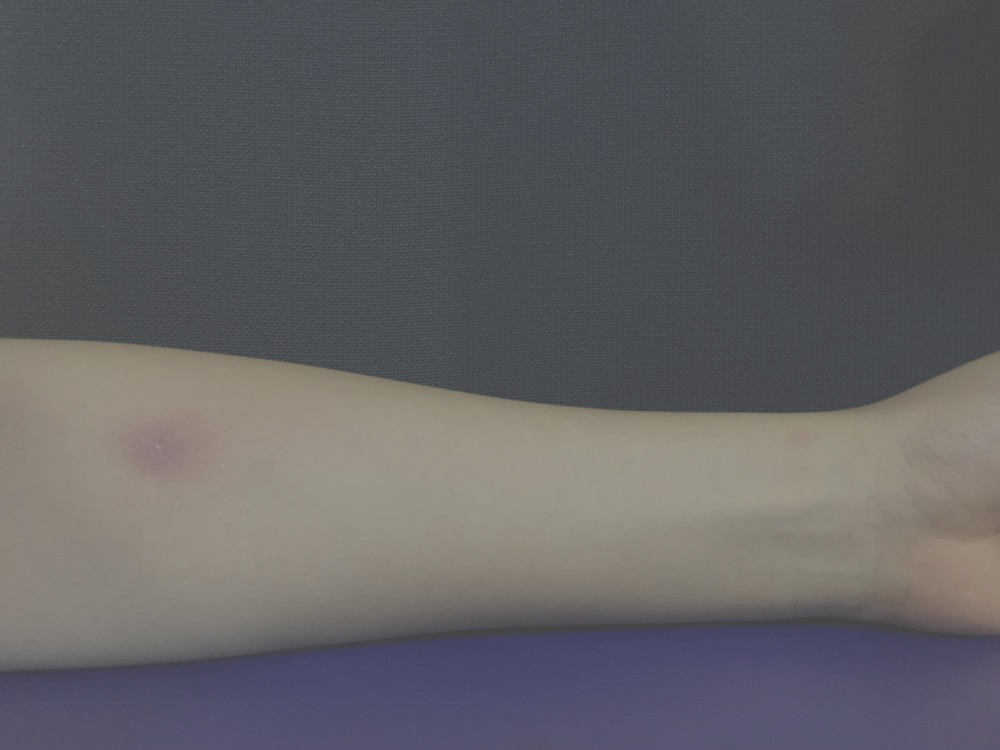
\includegraphics[scale=0.14]{img/contrast1}
  \caption{Reduce Contrast}
  \label{fig:sub1}
\end{subfigure}%
\begin{subfigure}{.3\textwidth}
  \centering
  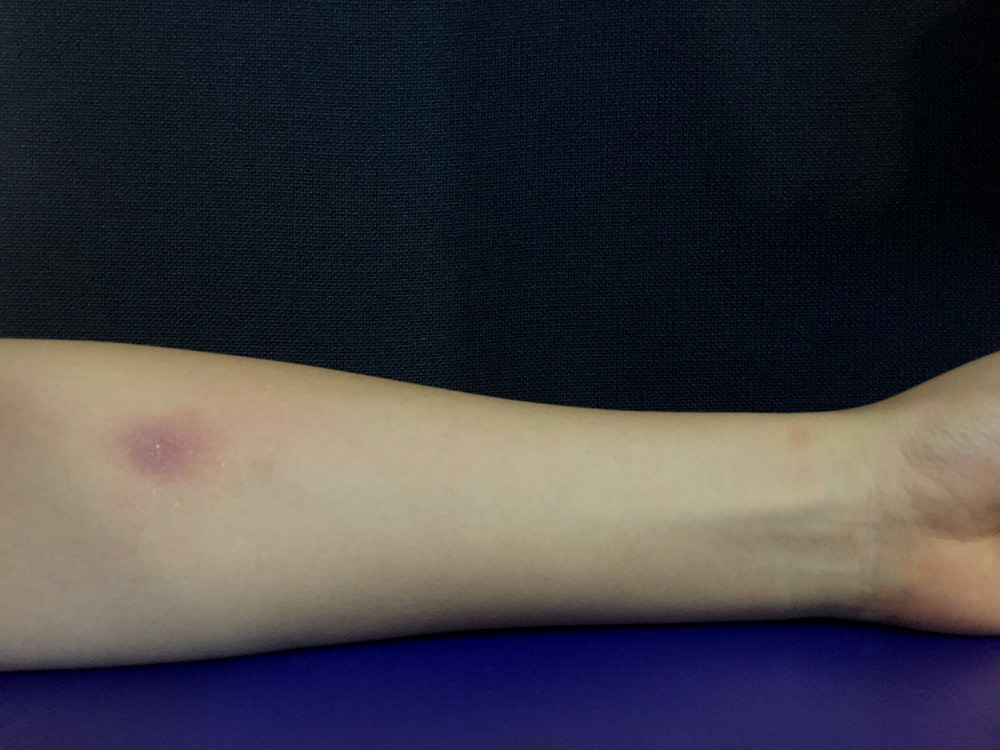
\includegraphics[scale=0.14]{img/original}
  \caption{Original Image}
  \label{fig:sub2}
\end{subfigure}
\begin{subfigure}{.3\textwidth}
  \centering
  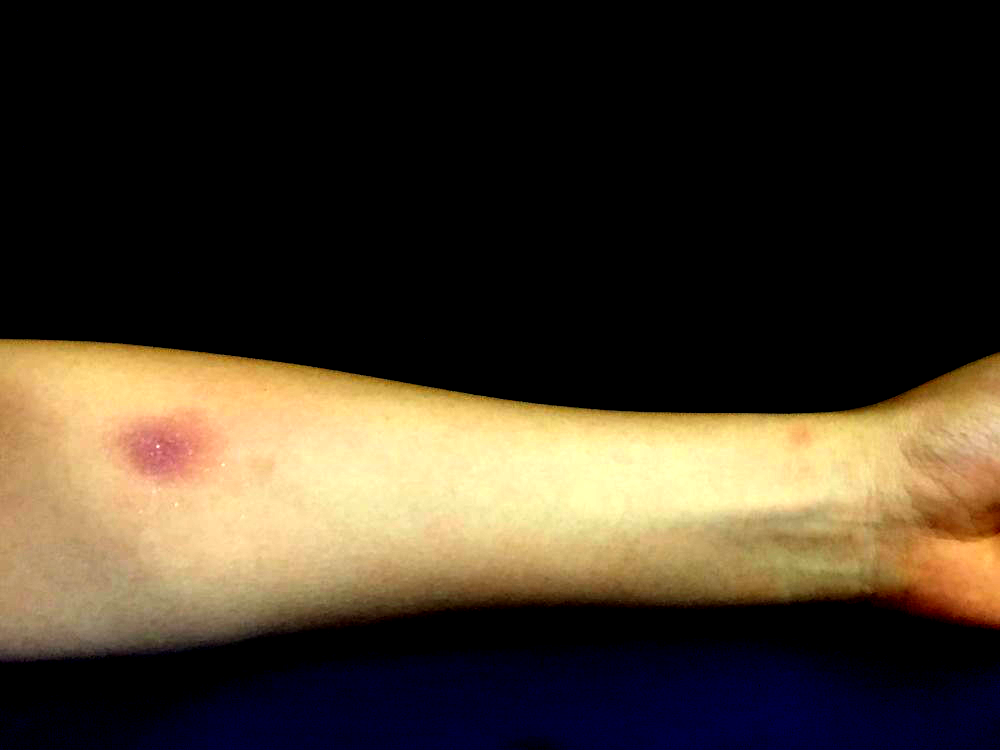
\includegraphics[scale=0.14]{img/contrast2}
  \caption{Add Contrast}
  \label{fig:sub2}
\end{subfigure}
\caption{Reduce and Add Contrast of the Image}
\label{fig:test}
\end{figure}

And the user also could adapt the brightness and contrast parameter to enhance different images, like Figure 5.4.
\begin{figure}[!htb]
	\centering
	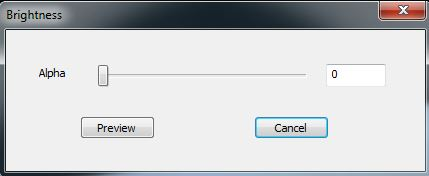
\includegraphics[scale=1]{img/brightdialog2}
	\caption{Brightness dialog}
\end{figure}
\section{Histogram}
In digital photography, the best feedback for evaluating an image is the histogram. A histogram is a graph that shows frequency. Usually histogram have bars that represent the frequency of occurring of data in the whole data set.   

\subsection{RGB Histogram}
Image Histogram is histogram  that acts as a graphical representation of the tonal distribution in a digital image.\cite{Sutton} For color images, it is presented the higtograms of red, green and blue channels. One of application of histogram is for brightness and contrast purpose. In the meantime, it is also used to detect pressure ulcers area, which will be discussed in the following sections. Figure 5.5 shows RGB Histogram diagram of the image.
\begin{figure}[h!]
	\centering
	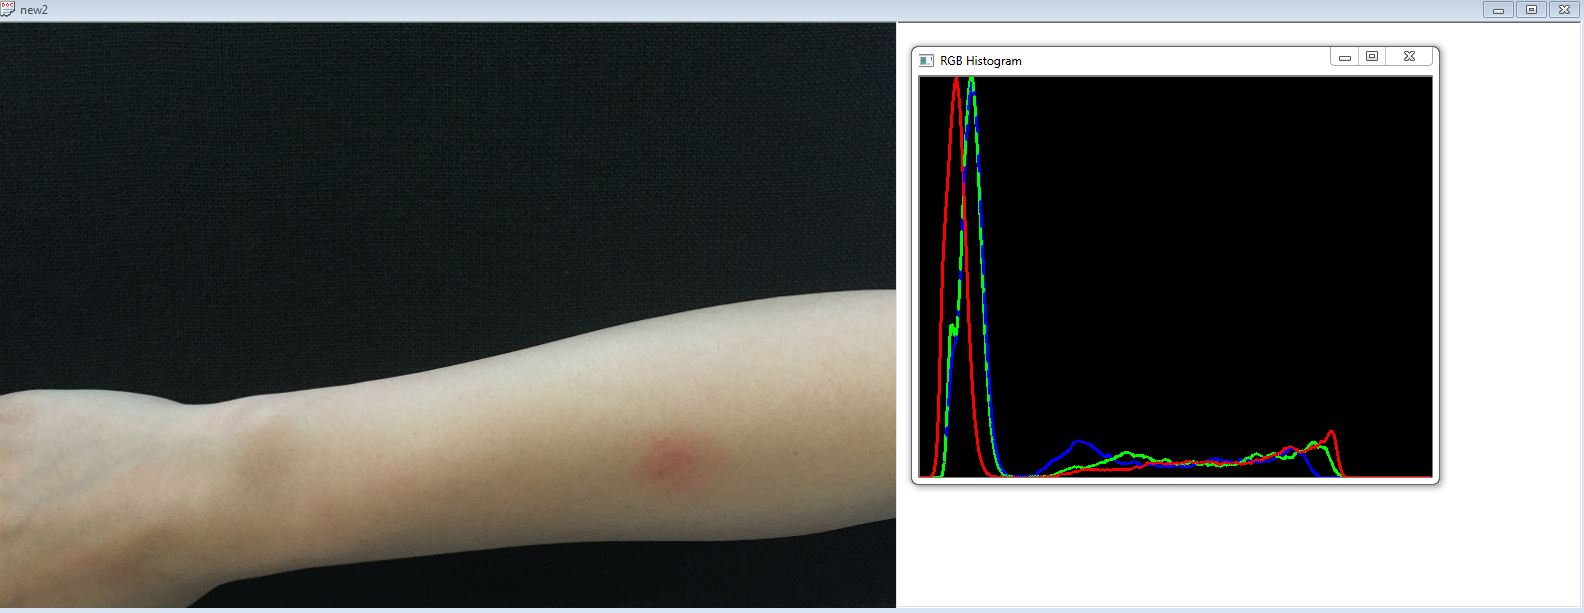
\includegraphics[scale=0.39]{img/rgbhistorgram}
	\caption{RGB Historgram}
\end{figure}

\newpage
\subsection{Histogram Equalization}
Histogram Equalization is to equalize flattening the intensity distribution curve or the intensity distribution of an image. And histogram equalization improves the contrast of an image. \\

In histogram equalization\cite{Gonzalez}, the dynamic range and contrast of an image is modified by altering the image such that its intensity histogram has a desired shape, which is achieved by using the cumulative distribution function as mapping function. The intensity levels are changed, for example, the peaks of the histogram are stretched, and the troughs are compressed. For the histogram $H(i)$, its cumulative distribution $H^{'}(i)$ is:
\begin{displaymath}
H^{'}(i)  = \sum_{0\leq j< i}^{} H(j)
\end{displaymath}
Then normalize $H^{'}(i)$ such that the maximum value is 255 ( or the maximum value for the intensity of the image ). Figure 5.6 shows the process of histogram equlization.

\begin{figure}[h!]
	\centering
	\includegraphics[scale=0.58]{img/histo}
	\caption{RGB Historgram}
\end{figure}

\newpage
It equalize the histogram of the intensity component only, not the color components. So, RGB format cannot be used because its all three planes represent color components blue, green and red. So it is necessary to convert the original BGR color space to YCrCb color space because its 1st plane represents the intensity of the image where as other planes represent the color components. Figure 5.4 shows the difference between the original image and image after histogram equalization.

\begin{figure}[!h]
\centering
\begin{subfigure}{.5\textwidth}
  \centering
  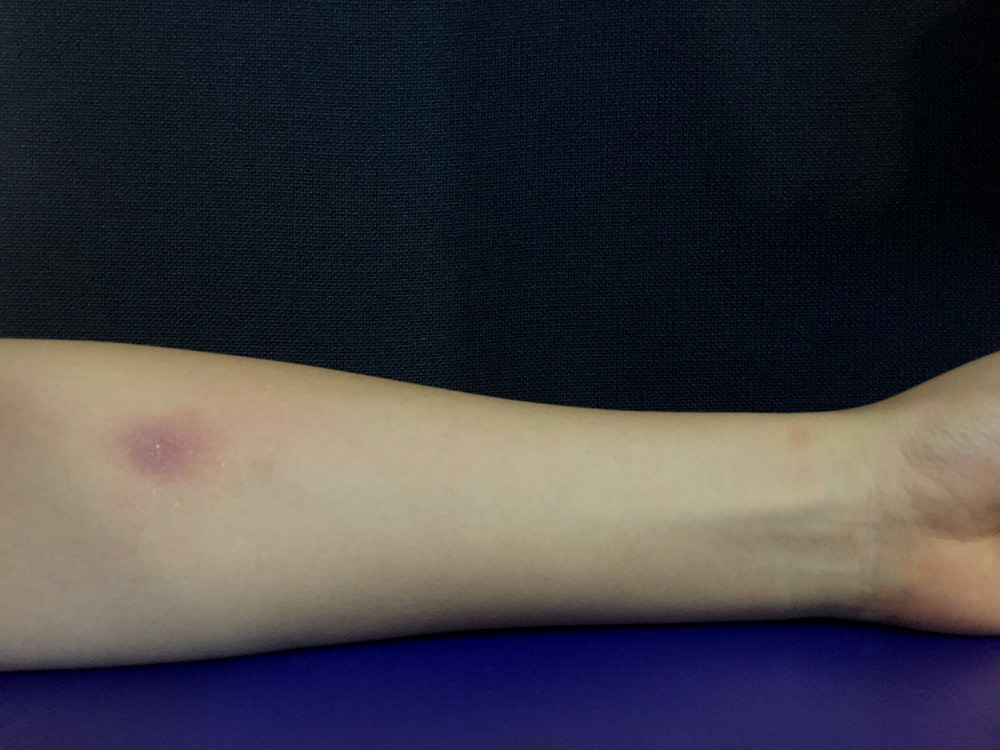
\includegraphics[scale=0.23]{img/original}
  \caption{Original Image}
  \label{fig:sub1}
\end{subfigure}%
\begin{subfigure}{.5\textwidth}
  \centering
  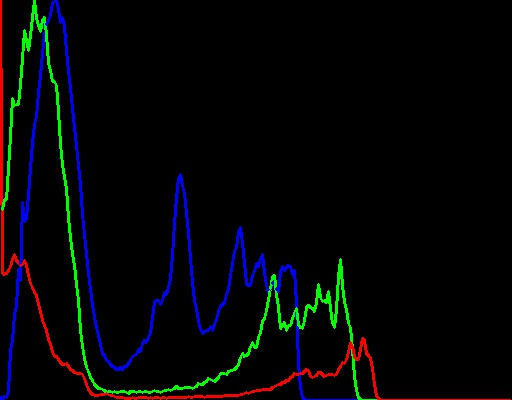
\includegraphics[scale=0.43]{img/image}
  \caption{RGB Histogram of Original Image}
  \label{fig:sub1}
\end{subfigure}
\begin{subfigure}{.5\textwidth}
  \centering
  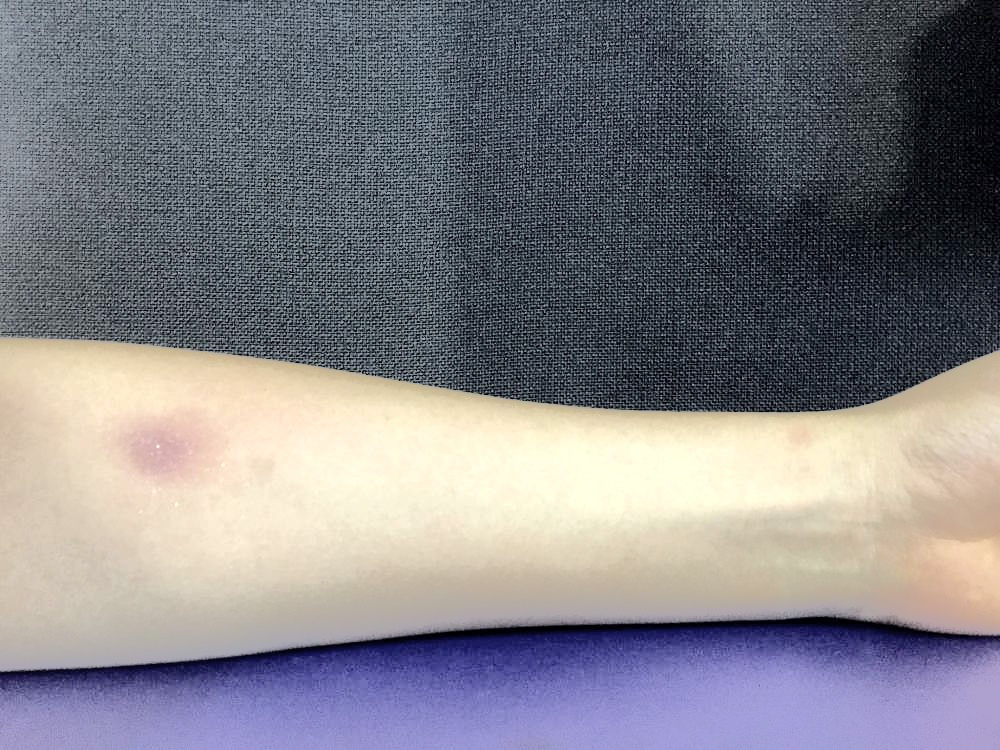
\includegraphics[scale=0.23]{img/equalize}
  \caption{Image After Histogram Equalization}
  \label{fig:sub2}
\end{subfigure}%
\begin{subfigure}{.5\textwidth}
  \centering
  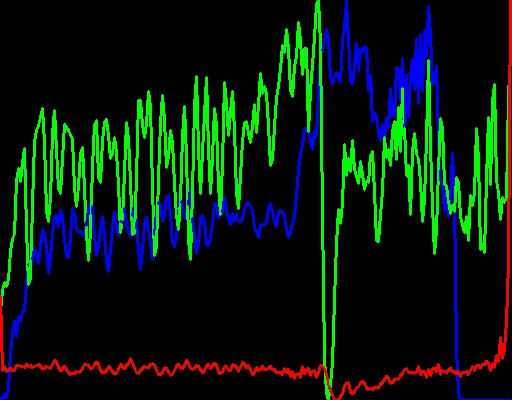
\includegraphics[scale=0.43]{img/equalimage}
  \caption{RGB Histogram of Result Image}
  \label{fig:sub1}
\end{subfigure}
\label{fig:test}
\caption{Image After Histogram Equalization}
\end{figure}
As Figure 5.7 shows, the new image contrast has been enhanced and its histogram has also been equalized. And during histogram equalization the overall shape of the histogram changes, where as in histogram stretching the overall shape of histogram remains same.

\subsection{Contrast Limited Adaptive Equalizaiton (CLAHE)}
Histogram equalization is suitable when histogram of the image is confined to a particular region. It won't work well when there is large intensity variations where the histogram covers a large region, such as both bright and dark pixels are present. \\

It is true that the background contrast has improved after histogram equalization. But compare the face of statue in both images. It may lost most of the information due to over-brightness, which is because that its histogram is not confined to a particular region.\\

In order to solve this problem, adaptive histogram equalization is used \cite{Pizer}.  It computes ordinary histograms, each one analogous with a section of the image.  However, Adaptive Histogram Equalization is responsible for over-amplifying noise in some homogeneous regions of an image. To avoid this drawback, Contrast Limited
Adaptive Histogram Equalization (CLAHE) is introduced \cite{clahe}\cite{Stark}.\\

In this way, image is divided into small blocks called "tiles", which is 8x8 by default in OpenCV 3.0. Then each of these blocks are histogram equalized as usual. Therefore, in a small area, histogram would confine to a small region. If there is noise, it will be amplified. To avoid this, contrast limiting is applied. If any histogram bin is the specified contrast limit, those pixels will be clipped and distributed uniformly to other bins before applying histogram equalization. After histogram equalization, apply the bilinear interpolation to remove artifacts in tile borders. Figure 5.8 shows CLAHE Process diagram.\\
\begin{figure}[!htb]
	\centering
	\includegraphics[scale=0.6]{img/CLAHEprocess}
	\caption{ Contrast Limited Adaptive Equalizaiton Process}
\end{figure}

And Note that CLAHE is only effective for images which contain relatively homogenous ere enhanced noise or artifacts may appear due to AHE. Following is the example images where performing CLAHE is effective.

\begin{figure}[!h]
\centering
\begin{subfigure}{.5\textwidth}
  \centering
  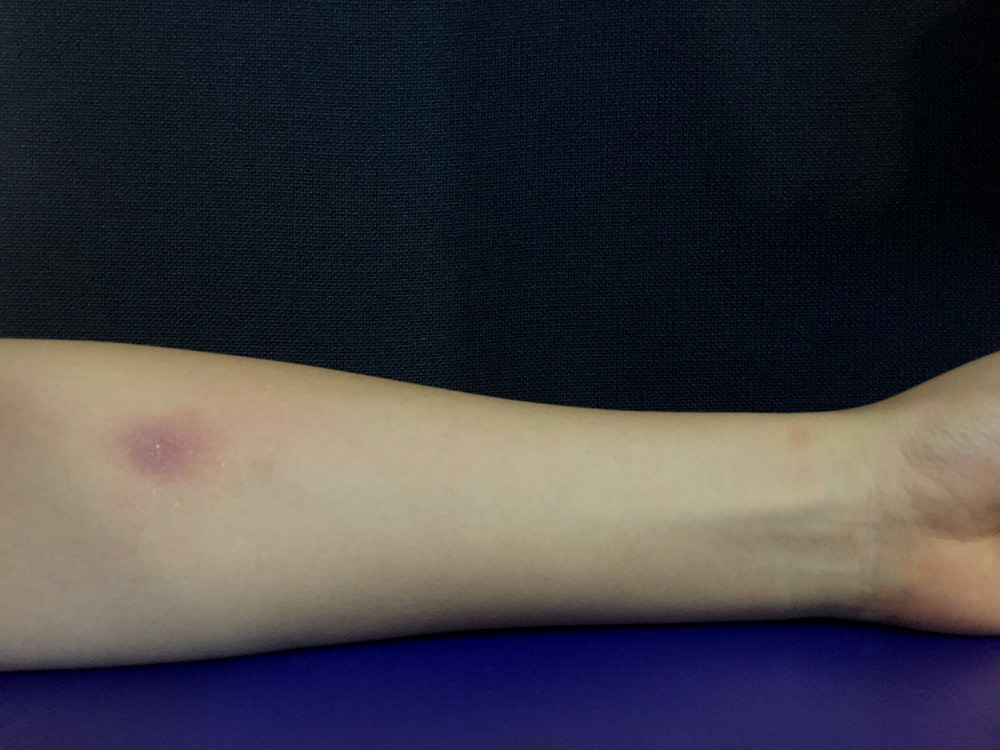
\includegraphics[scale=0.23]{img/original}
  \caption{Original Image}
  \label{fig:sub1}
\end{subfigure}%
\begin{subfigure}{.5\textwidth}
  \centering
  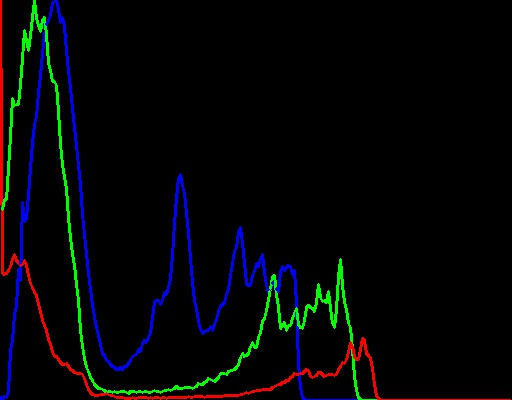
\includegraphics[scale=0.43]{img/image}
  \caption{RGB Histogram of Original Image}
  \label{fig:sub1}
\end{subfigure}
\begin{subfigure}{.5\textwidth}
  \centering
  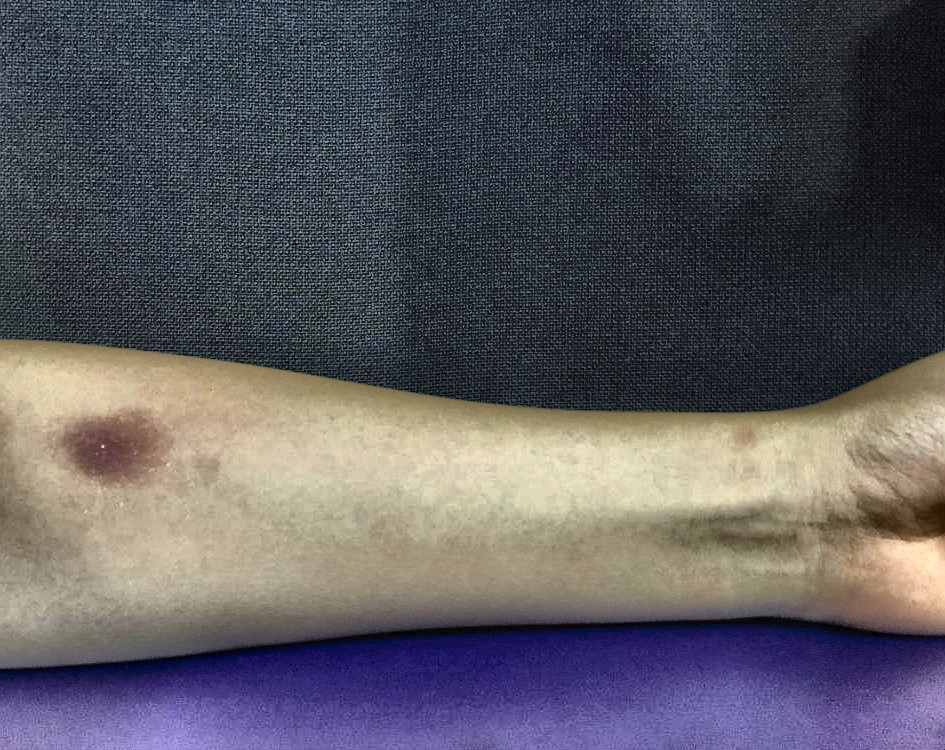
\includegraphics[scale=0.23]{img/cla2}
  \caption{Image After CLAHE}
  \label{fig:sub2}
\end{subfigure}%
\begin{subfigure}{.5\textwidth}
  \centering
  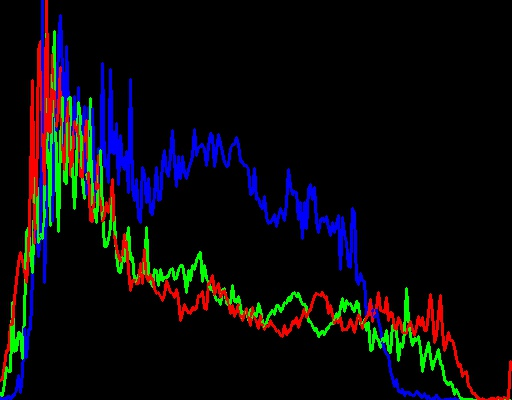
\includegraphics[scale=0.43]{img/imagecla}
  \caption{RGB Histogram of Result Image}
  \label{fig:sub1}
\end{subfigure}
\label{fig:test}
\caption{Image After Contrast Limited Adaptive Equalizaiton(CLAHE)}
\end{figure}

\newpage
\section{Image Filter}
Image processing filters \cite{Jain}, also called image blur, are mainly used to suppress either the high frequencies in the image, such as smoothing the image, or enhancing or detecting edges in the image. Images can be filtered either in the spatial domain or  in the frequency.

\subsection{Median Filter}
The median filter is used to reduce noise in an image, and compared with the median filter of preserving useful detail in the imag, it often does a better job.\\

A template of size 3x3, 5x5, 7x7,… etc is applies to each pixel. The values within the template are sorted and the middle of the sorted list is used to replace the templates central pixel. Figure 5.10 shows how does median filter work\cite{computervision}.
\begin{figure}[!htb]
	\centering
	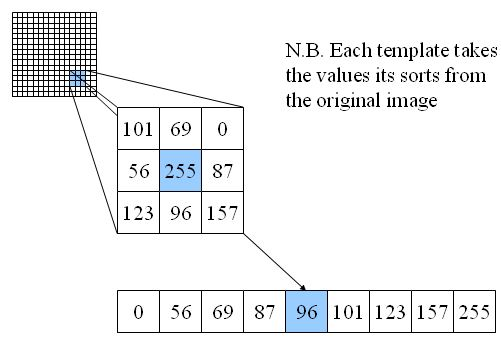
\includegraphics[scale=0.8]{img/medianfilterprocess}
	\caption{ How median filter works?}
\end{figure}


\newpage
 The input image is convolved with a Median kernel. Median filtering is widely used in edge detection algorithms because under certain conditions, it preserves edges while removing noise. Figure 5.9 shows the differences between the original image and image after median filter.
\begin{figure}[!h]
\centering
\begin{subfigure}{.5\textwidth}
  \centering
  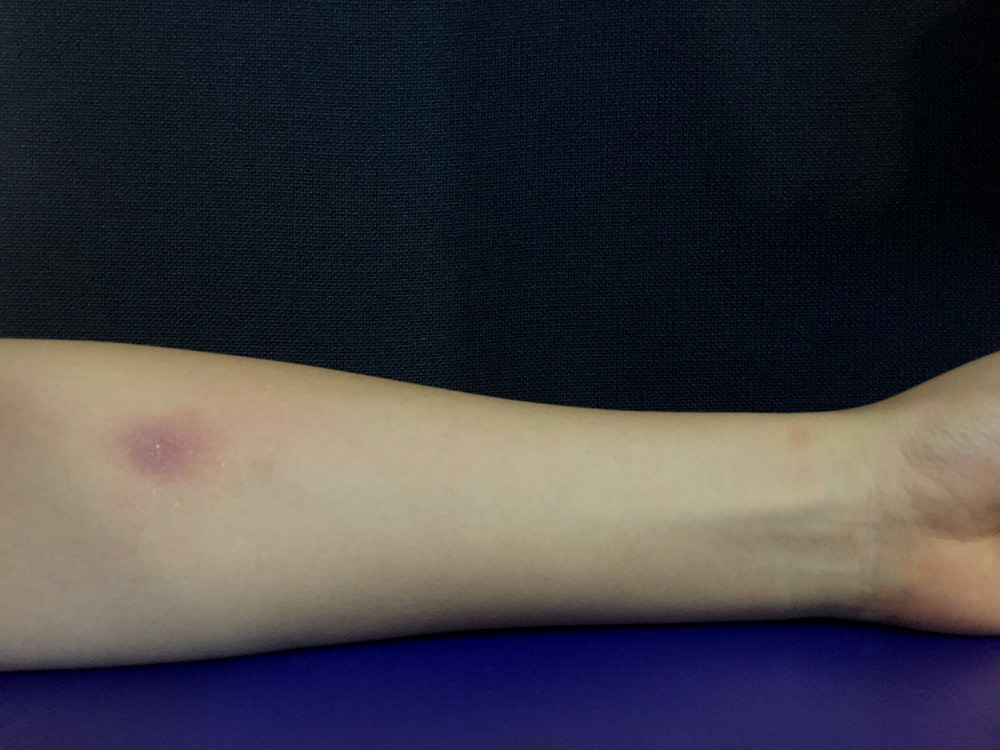
\includegraphics[scale=0.23]{img/original}
  \caption{Original Image}
  \label{fig:sub1}
\end{subfigure}%
\begin{subfigure}{.5\textwidth}
  \centering
  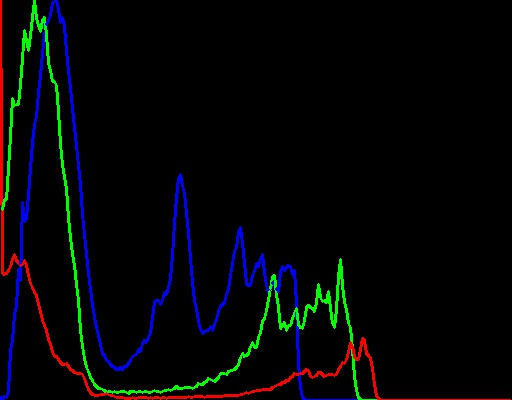
\includegraphics[scale=0.43]{img/image}
  \caption{RGB Histogram of Original Image}
  \label{fig:sub1}
\end{subfigure}
\begin{subfigure}{.5\textwidth}
  \centering
  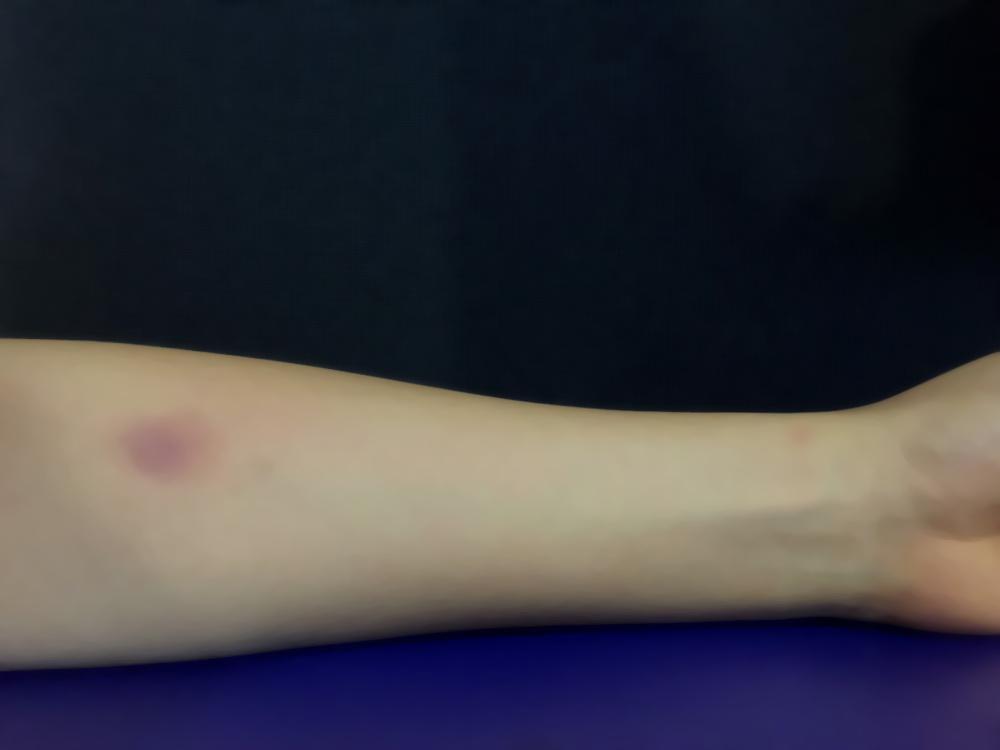
\includegraphics[scale=0.23]{img/filter}
  \caption{Image After Median Filter}
  \label{fig:sub2}
\end{subfigure}%
\begin{subfigure}{.5\textwidth}
  \centering
  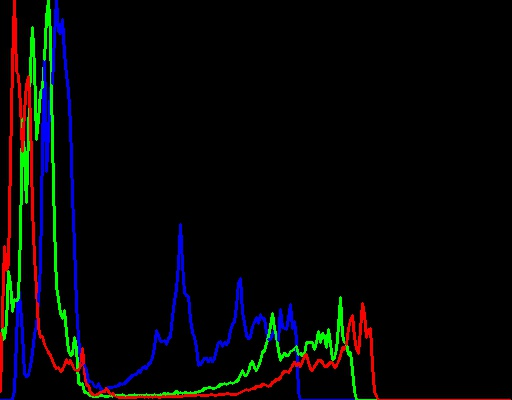
\includegraphics[scale=0.43]{img/medianrgb}
  \caption{RGB Histogram of Result Image}
  \label{fig:sub1}
\end{subfigure}
\label{fig:test}
\caption{Image After Median Filter}
\end{figure}
  
\subsection{Gaussian Filter}
The Gaussian smoothing is a 2D convolution operator, which is used to blur images and remove noises and details. In this sense it is similar to mean filter, but it uses different kernels that represent the shape of a Gaussian hump. \\

In 2D, an isotropic Gaussian has the form:
\begin{displaymath}
G\left ( x,y \right ) = \frac{1}{2\pi \delta ^{2}}e^{-\frac{x^{2}+y^{2}}{2\delta ^{2}}}
\end{displaymath}

Where $\delta$ is the standard deviation of the distribution. The distribution is assumed to have a mean of 0.\\

The idea of Gaussian smoothing is to use the 2D distribution as a point-spread function. And the image needs to produce a discrete approximation to the Gaussian function before performing the convolution. In theory, the Gaussian distribution is non zero everywhere, which will require an infinitely large convolution kernel, in practice it is effectively zero more than three standard deviations from the mean, and therefore we can truncate the kernel at this point. Figure 5.12 shows a suitable integer-valued convolution kernel that approximates a Gaussian with a $\delta$ of 1.0. The value of the Gaussian over the whole pixel is integrated. And 273 is the sum of all the values in the mask.\\

\begin{figure}[!htb]
	\centering
	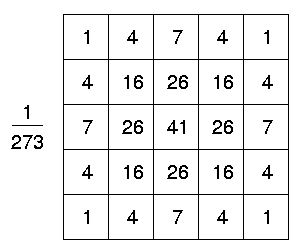
\includegraphics[scale=0.9]{img/gaussianmat}
	\caption{Discrete approximation to Gaussian function with $\delta$=1.0}
\end{figure}


\begin{figure}[!h]
\centering
\begin{subfigure}{.5\textwidth}
  \centering
  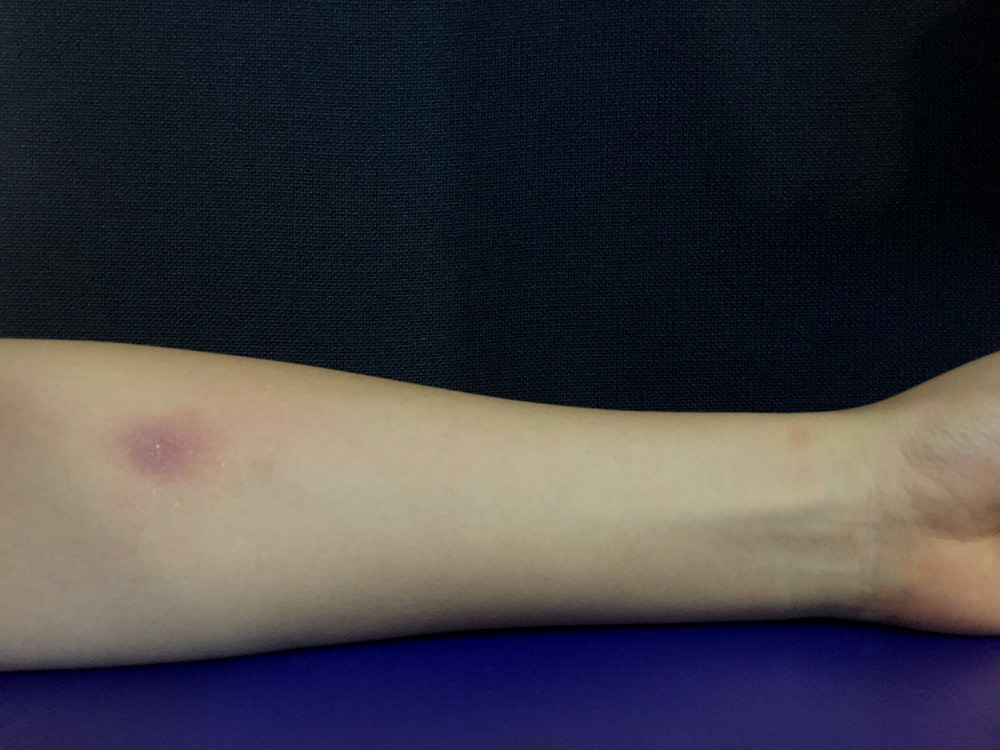
\includegraphics[scale=0.23]{img/original}
  \caption{Original Image}
  \label{fig:sub1}
\end{subfigure}%
\begin{subfigure}{.5\textwidth}
  \centering
  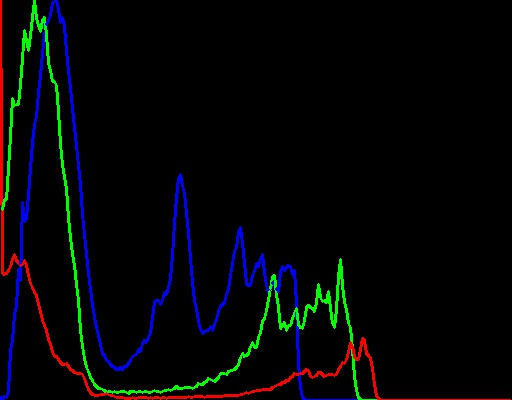
\includegraphics[scale=0.43]{img/image}
  \caption{RGB Histogram of Original Image}
  \label{fig:sub1}
\end{subfigure}
\begin{subfigure}{.5\textwidth}
  \centering
  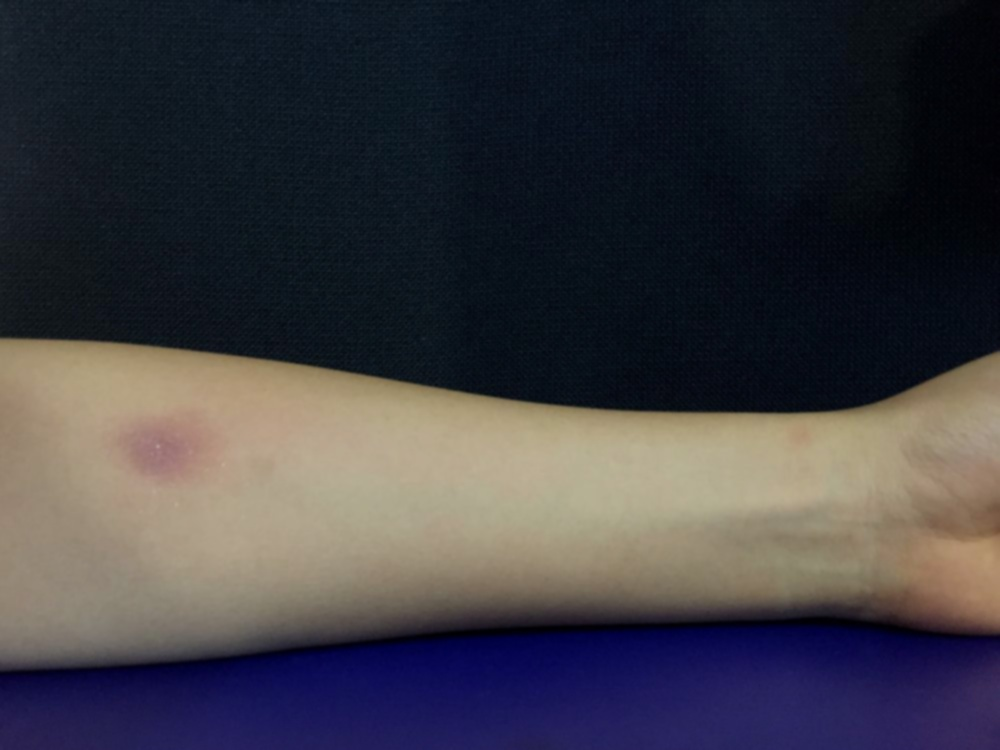
\includegraphics[scale=0.23]{img/gaussian}
  \caption{Image After Gaussian Filter}
  \label{fig:sub2}
\end{subfigure}%
\begin{subfigure}{.5\textwidth}
  \centering
  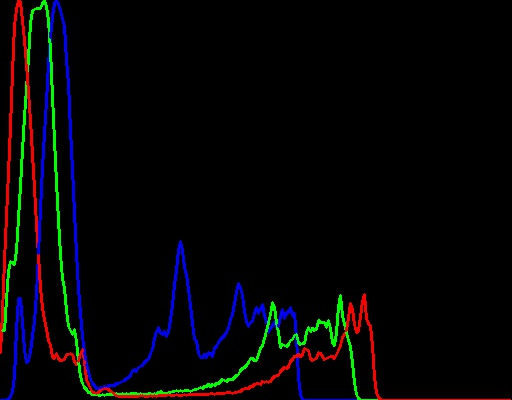
\includegraphics[scale=0.43]{img/gaussianrgb}
  \caption{RGB Histogram of Result Image}
  \label{fig:sub1}
\end{subfigure}
\label{fig:test}
\caption{Image After Gaussian Filter}
\end{figure}

Gaussian Filter is also used to reduce noises in an image. Gaussian kernel is slided across the image to produce the smoothed image. The size of the kernel and the standard deviation of the Gaussian distribution in X and Y direction should be chosen carefully. Figure 5.13 shows the differences between the original image and image after gaussian filter.

\newpage
\subsection{Bilateral Filter}
 All of the above filters smooth away the edges while removing noises. But Bilateral filter can reduce noises of the image while preserving the edges. Similarly to the Gaussian convolution, the bilateral filter is defined as a weighted average of pixels. The difference is that the bilateral filter takes into account the variation of intensities to preserve edges. The rationale of bilateral filtering is that two pixels are close to each other not only if they occupy nearby spatial locations but also if they have some similarity in the
photometric range \cite{Paris}.\\

The formalization goes back in the literature to Yaroslavsky \cite{Yaroslavsky}, then Aurich
and Weule \cite{Aurich}, Smith and Brady \cite{Smith} and Tomasi and Manduchi \cite{Tomasi}. The bilateral filter, denoted is defined as:
 
\begin{displaymath}
BF\left [ I \right ]_{p} = \frac{1}{W_{p}}\sum_{q\in S}^{q}G_{\delta _{s}}\left ( \left \| p-q \right \| \right )G_{\delta _{r}}\left ( I_{p}-I_{q} \right )I_{q}
\end{displaymath}

where $W_{p}$ is a normalization factor:
\begin{displaymath}
BF\left [ I \right ]_{p} = \frac{1}{W_{p}}\sum_{q\in S}^{q}G_{\delta _{s}}\left ( \left \| p-q \right \| \right )G_{\delta _{r}}\left ( I_{p}-I_{q} \right )I_{q}
\end{displaymath}

Parameters $\sigma _{s}$ and $\sigma _{r}$ measures the amount of filtering for the image I. $W_{p}$ normalizes weighted average where $G_{\sigma _{s}}$ is a spatial Gaussian that decreases the influence of
distant pixels, $G_{\sigma _{r}}$ a range Gaussian that decreases the influence of pixels $q$ with an intensity
value different from $I_{q}$. The term range qualifies quantities related to pixel values, by opposition to space which refers to pixel location. Figure 5.14 shows the differences between the original image and image after bilateral filter. And the disadvantage of bilateral filter is that it takes longer time to process.
\begin{figure}[!h]
\centering
\begin{subfigure}{.5\textwidth}
  \centering
  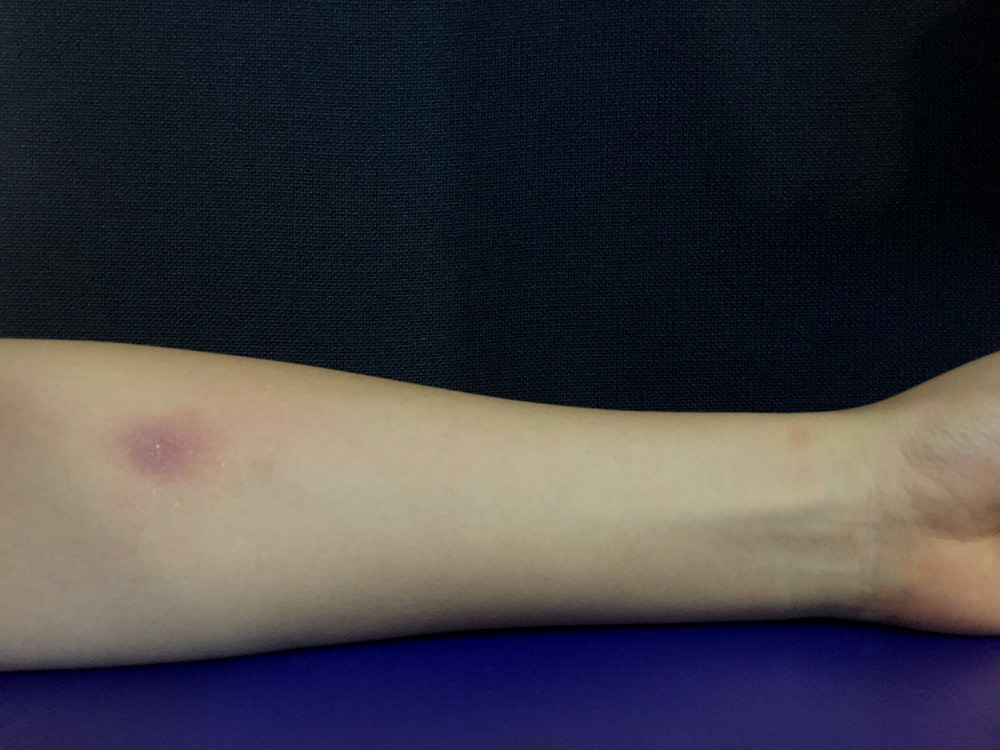
\includegraphics[scale=0.23]{img/original}
  \caption{Original Image}
  \label{fig:sub1}
\end{subfigure}%
\begin{subfigure}{.5\textwidth}
  \centering
  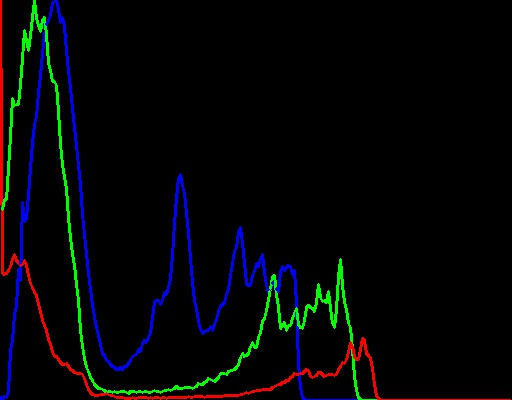
\includegraphics[scale=0.43]{img/image}
  \caption{RGB Histogram of Original Image}
  \label{fig:sub1}
\end{subfigure}
\begin{subfigure}{.5\textwidth}
  \centering
  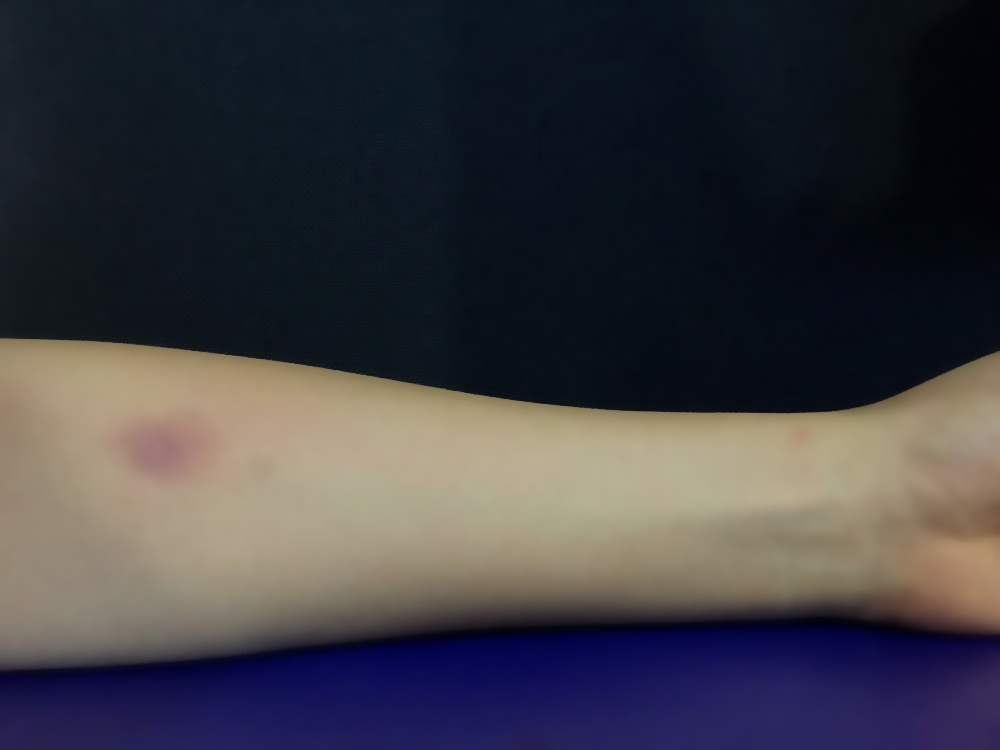
\includegraphics[scale=0.23]{img/bilateral}
  \caption{Image After Bilateral Filter}
  \label{fig:sub2}
\end{subfigure}%
\begin{subfigure}{.5\textwidth}
  \centering
  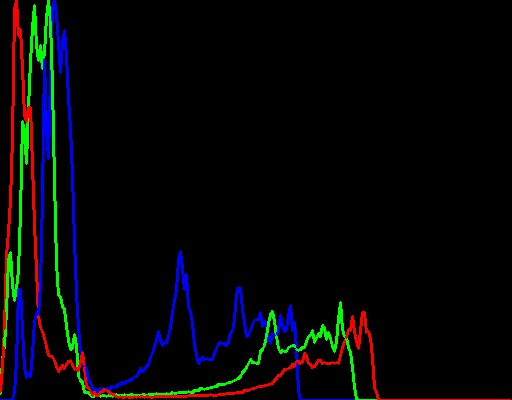
\includegraphics[scale=0.43]{img/bilterrgb}
  \caption{RGB Histogram of Result Image}
  \label{fig:sub1}
\end{subfigure}
\label{fig:test}
\caption{Image After Bilateral Filter}
\end{figure}


\section{Detect Pressure Ulcers Area}
In order to detect the pressure ulcers area, using contours as a curve joinging all the continuous points, having the same color(which is red in this case). Contour tracing is a technique that is applied to digital images in order to extract their boundary. Figure 5.15 shows the process of Contour tracing pressure uclers area. 
\begin{figure}[!htb]
	\centering
	\includegraphics[scale=0.7]{img/detectprocess}
	\caption{Pressure ulcers area detection process}
\end{figure}

\newpage
\subsubsection{input image}
Usually it is RGB image. Figure 5.16 is the original image. This part starts with two different input images to show how this alogorithm works.
 \begin{figure}[!htb]
\centering
\begin{subfigure}{.5\textwidth}
  \centering
  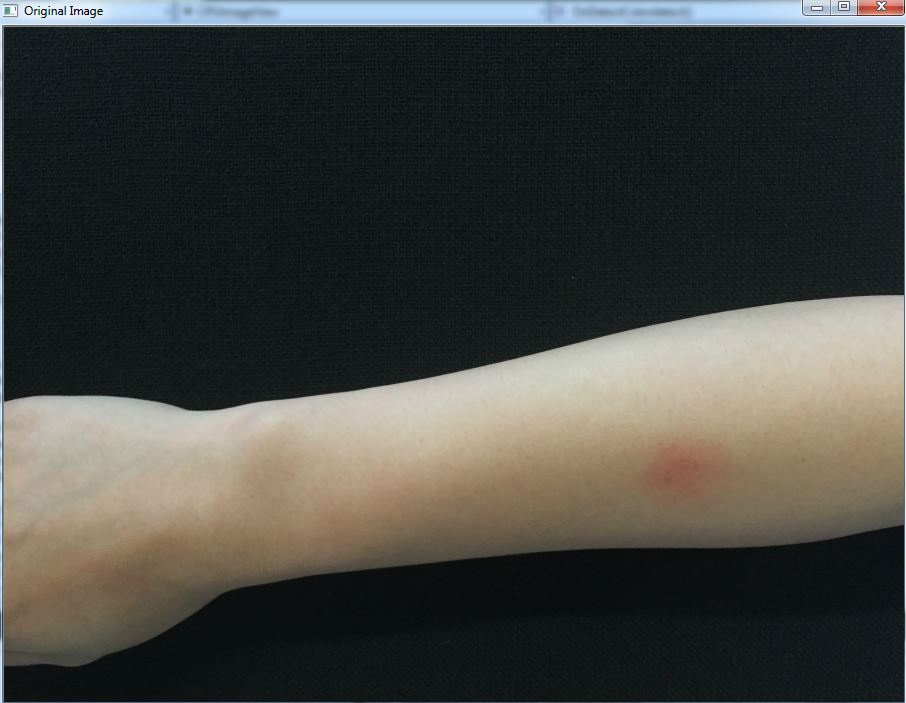
\includegraphics[width=8cm,height=6cm]{img/detectoringinal}
  \caption{Original Image1}
  \label{fig:sub1}
\end{subfigure}%
\begin{subfigure}{.5\textwidth}
  \centering
  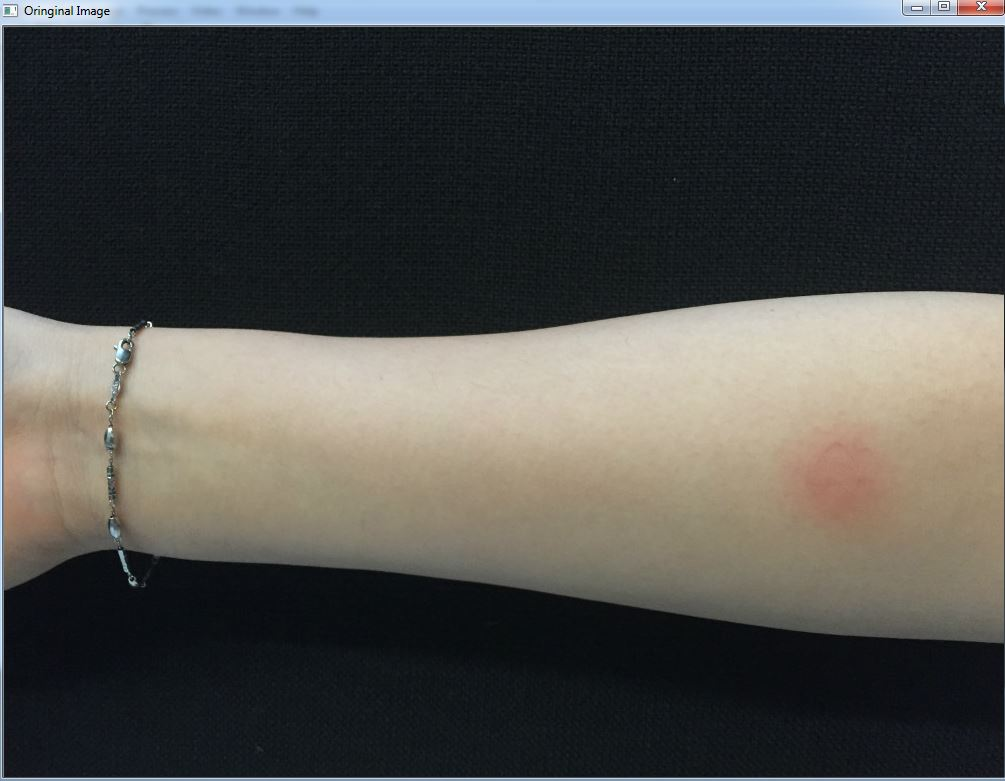
\includegraphics[width=8cm,height=6cm]{img/detectoringinal2}
  \caption{Original Image2}
  \label{fig:sub2}
\end{subfigure}
\caption{Original Image Input}
\label{fig:test}
\end{figure}


\newpage
\subsubsection{Median Filter}
As section 5.4 discribe median filter, apparently the noise from the input image fooled the Hough detector. So a cure is to filter the input image before the RGB to HSV conversion, for this kind of noise usually a median filter works best. And then transfer the RGB format to HSV to get the hue value. However, Median Filter smooths away the edges while removing noises
 \begin{figure}[!h]
\centering
\begin{subfigure}{.5\textwidth}
  \centering
  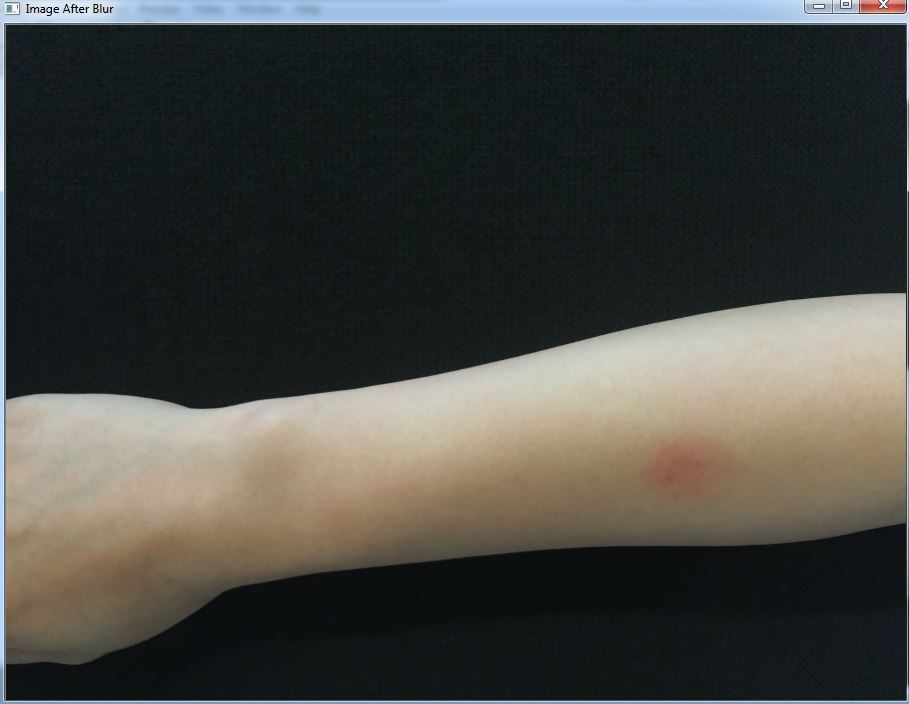
\includegraphics[width=8cm,height=6cm]{img/detectfilter}
  \caption{Image1 After Median Filter}
  \label{fig:sub1}
\end{subfigure}%
\begin{subfigure}{.5\textwidth}
  \centering
  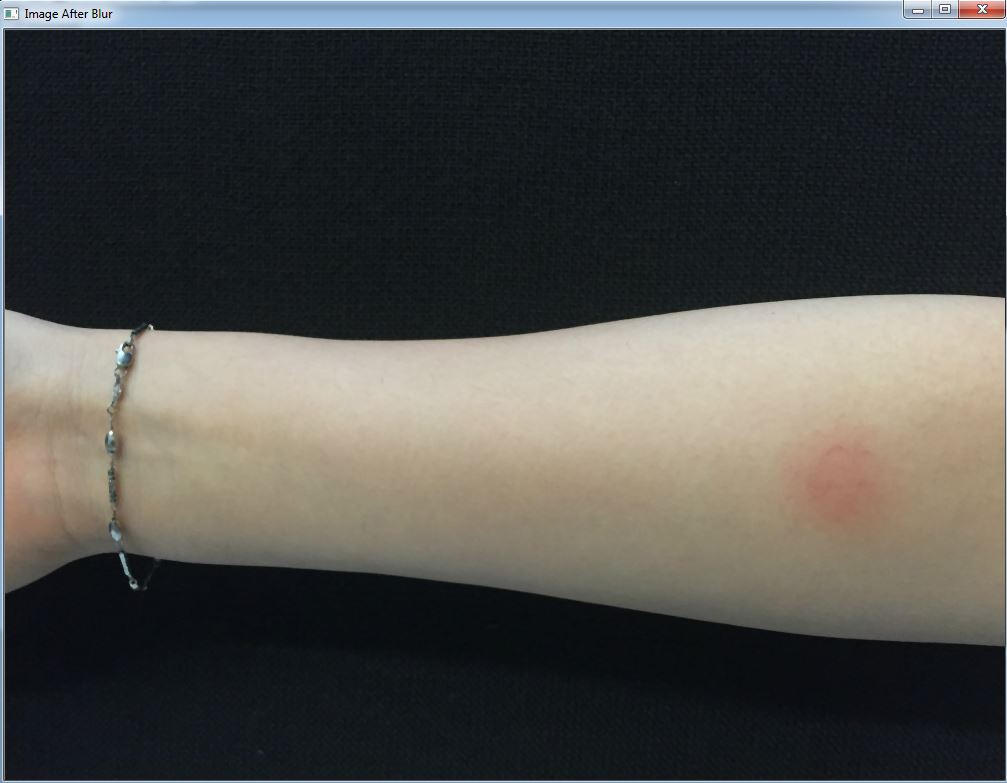
\includegraphics[width=8cm,height=6cm]{img/detectfilter2}
  \caption{Image2 After Median Filter}
  \label{fig:sub2}
\end{subfigure}
\caption{Image After Median Filter}
\label{fig:test}
\end{figure}

\subsubsection{Threshold}
Thresholding \cite{Zhang} is one of the commonest method of image segmentation. Thresholding is a simple but effective tool to separate objects from the background. This report uses fixed thresholding. If pixel value is greater than a threshold value, it is assigned one value or it may be white, else it is assigned another value or it may be black.\\

If $g(x, y)$ is a thresholded version of $f(x, y)$ at some global threshold $T$,
\[
    g(x,y)=\left\{
                \begin{array}{ll}
                  1 & if f(x,y)\geq T\\
                  0 & otherwise\\
                \end{array}
              \right.
  \]



Threshold the HSV image, keep only the red pixels, which is closer to the color of pressure ulcers skins. In this case, setting the hue values approximately in the range of 0 to 10. And compare threshold images and results image to show how saturation value to effect the detection result. Figure 5.16, setting saturation value ranges from 100 to 255. Figure 5.17, setting saturation value ranges from 95 to 255. The result shows that when the pressure is light, using the latter parameter will get the large area, however, it also detect the irrelevant area. So in this paper, setting the hsv value as 
Scalar(0, 98, 100) to Scalar(15, 255, 255). Explore the website: \url{http://colorizer.org/}
to get more color value details.\\

As Figure 5.19 shows, the result varies due to different global threshold $T$.

 \begin{figure}[!h]
\centering
\begin{subfigure}{.5\textwidth}
  \centering
  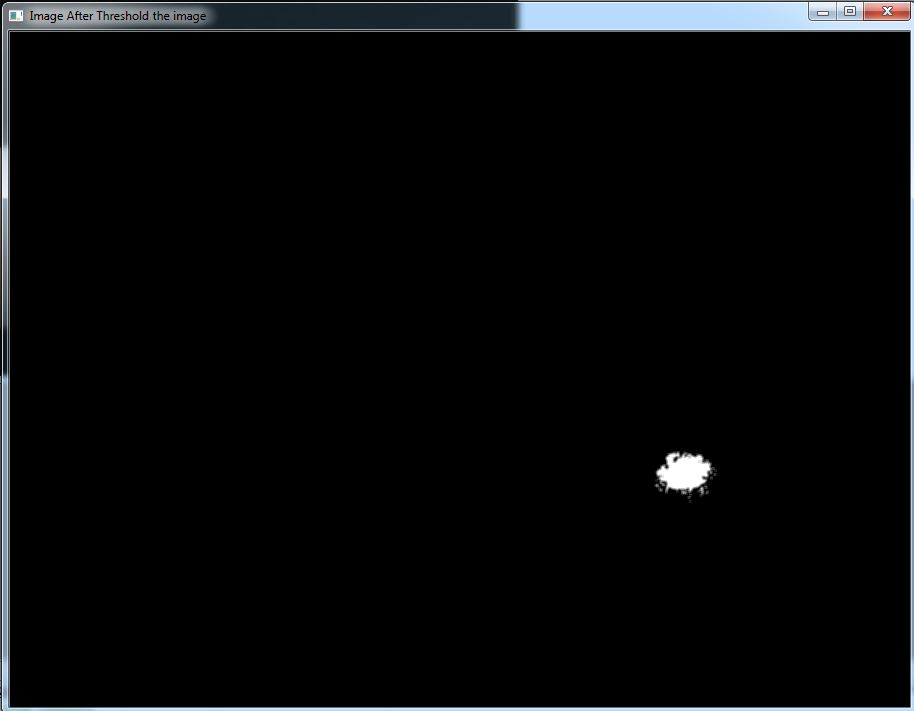
\includegraphics[width=8cm,height=6cm]{img/detectthreshold}
  \caption{Image1 After Threshold With s(100,255)}
  \label{fig:sub1}
\end{subfigure}%
\begin{subfigure}{.5\textwidth}
  \centering
  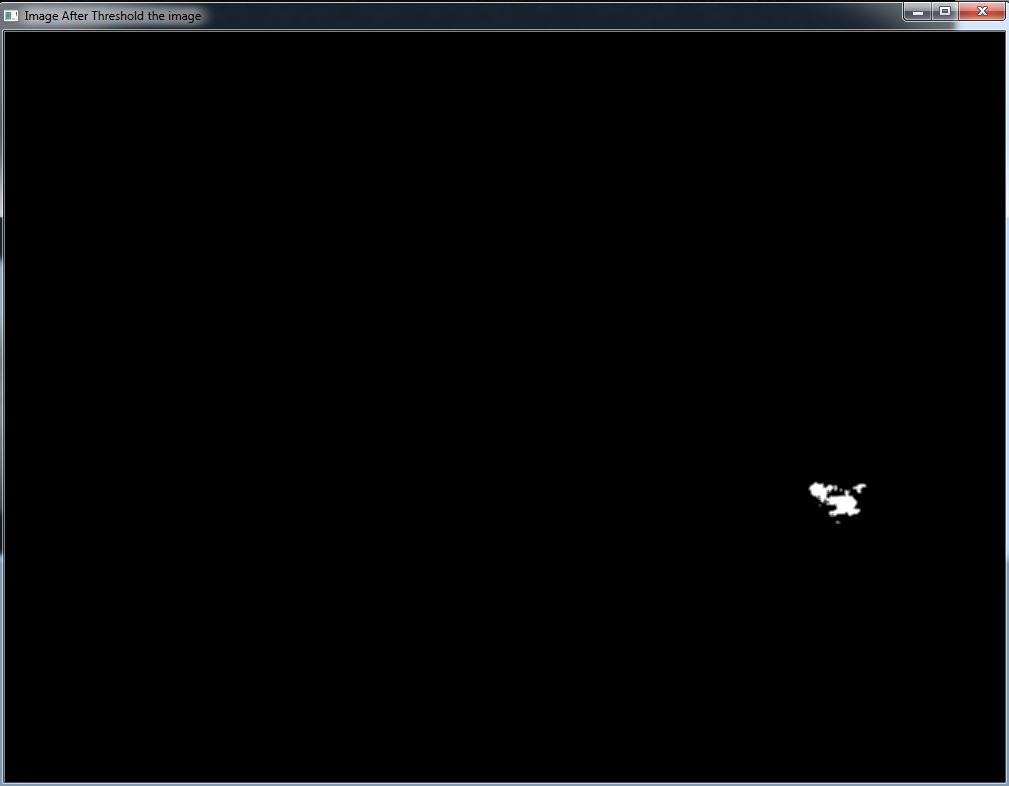
\includegraphics[width=8cm,height=6cm]{img/detectthreshold2}
  \caption{Image2 After Threshold With s(100,255)}
  \label{fig:sub2}
\end{subfigure}
\caption{Image After Threshold the filtered image With s(100,255)}
\label{fig:test}
\end{figure}

 \begin{figure}[!h]
\centering
\begin{subfigure}{.5\textwidth}
  \centering
  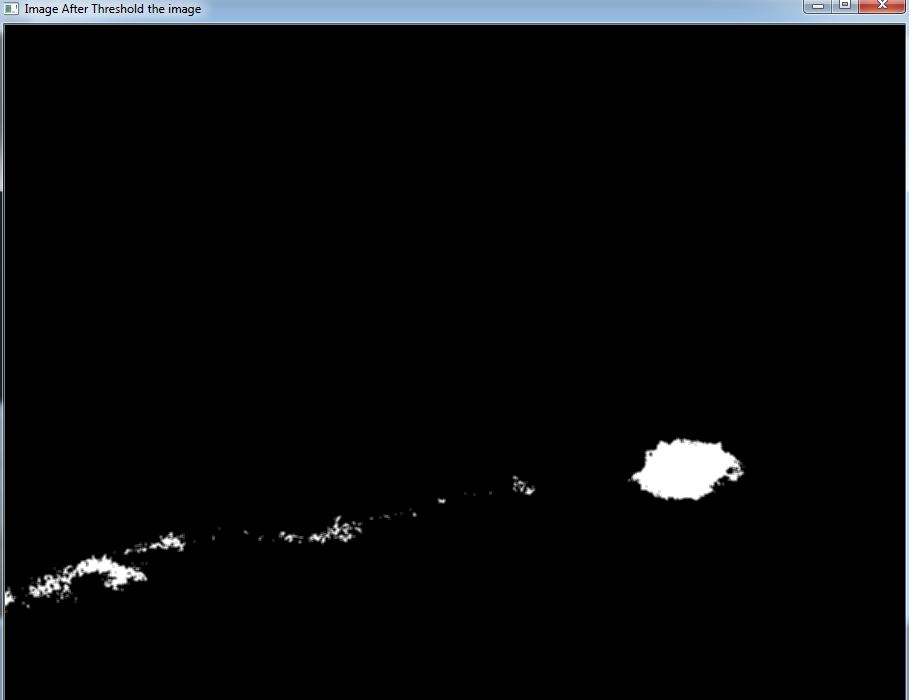
\includegraphics[width=8cm,height=6cm]{img/3}
  \caption{Image1 After Threshold With s(95,255)}
  \label{fig:sub1}
\end{subfigure}%
\begin{subfigure}{.5\textwidth}
  \centering
  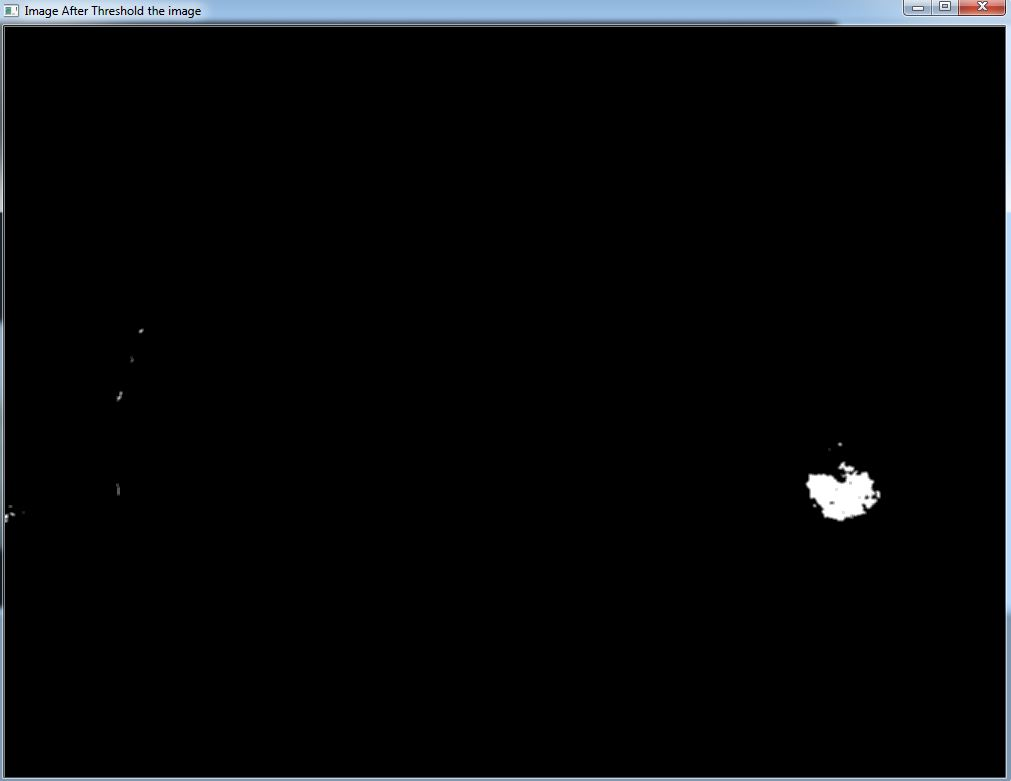
\includegraphics[width=8cm,height=6cm]{img/1}
  \caption{Image2 After Threshold With s(95,255)}
  \label{fig:sub2}
\end{subfigure}
\caption{Detect edges using Threshold Image With s(95,255)}
\label{fig:test}
\end{figure}

\newpage
\subsubsection{Contours}
The next step is to find the contours and draw approximate contours to polygons, and get bounding circles. Contour is defined as the curve joining all the continuous points, having same color or intensity. The contours are the useful tool for shape analysis and object detection and recognition.\\

For better accuracy, the report uses binary images. That's why thresholding is applied before. In OpenCV, finding contours is like finding white object from black background, and it can take images created by canny, which have edge pixels in them, or images created by thresholding,  in which the edge is implicit as boundaries between positive and negative regions. \\

It is necessary to understand the concept of a contour tree, which is significant to understand how findcontours() will communicate its result \cite{suzuki}.\\

\begin{figure}[!htb]
	\centering
	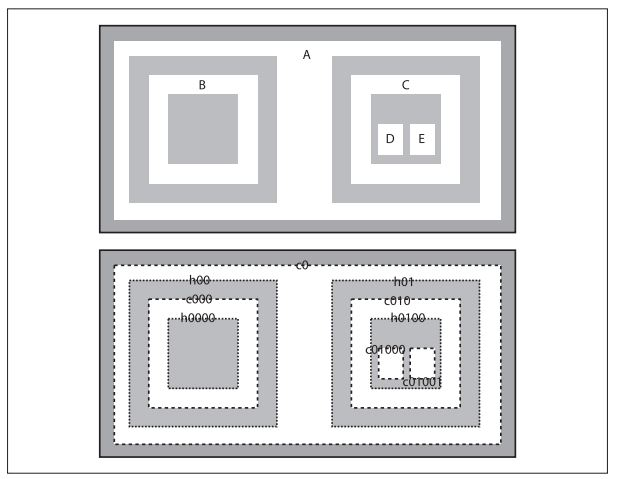
\includegraphics[scale=0.8]{img/conter}
	\caption{ A test image passed to findContours(): the found contours may be
either of two types, exterior “contours” (dashed lines) or “holes” (dotted lines)}
\end{figure}


\newpage
Figure 5.20 depicts the functionality of findContours(). The upper part shows an image containing a number of white regions on a dark background. The lower part depicts the same image along with the contours that will be located by the function. These contours are labeled $cX$ or $hX$, meaning contour hole and contour number. Some of those contours are dashed lines, which represents exterior
boundaries of the white regions (such as nonzero regions). OpenCV distinguishs between these exterior boundaries and the dotted lines\cite{Bradski}.Now look at the function in OpenCV, \\

void findContours(InputOutputArray image, OutputArrayOfArrays contours, OutputArray hierarchy, int mode, int method, Point offset=Point())\\

Parameters:	
\begin{itemize}
    \item image: Source, an 8-bit single-channel image. Images are treated as binary image, non-zero pixels are treated as 1’s and zero pixels remain 0’s.
    \item contours: Detected contours, which are stored as a vector of points.
    \item hierarchy: Optional vector, containing information about the image topology. For each contour $contours[i]$ , the elements hierarchy$[i][0]$ , $hiearchy[i][1]$, $hiearchy[i][2]$, and $hiearchy[i][3]$ are set to 0-based indices in contours of the previous and next contours at the same hierarchical level, the first child contour and the parent contour, respectively. If those parameter does not exist, the corresponding elements of hierarchy[i] is negative.
    \item mode: contour retrieval mode. This report chooses CV\_RETR\_TREE, which retrieves all of the contours and reconstructs a full hierarchy of nested contours.
    \item method: contour approximation method. This report chooses (CV\_CHAIN\_APPROX\_SIMPLE), compresses vertical, horizontal and diagonal segments and leaves only their end points.
\end{itemize}

For CV\_RETR\_TREE, that means that the root node is the outermost contour $c0$ showed in the Figure 5.20. Below $c0$ is the hole $h00$, which is connected to another hole $h01$ at the
same level. Each hole in turn has children $c000$ and $c010$ respectively, which are connected to their parents by vertical links. This continues down to the most-interior contours in the image, which become the leaf nodes in the tree.\\

Then the next tasks is to draw a contour using drawContours() function. And here extends drawing a circle based on the contours center. Figure 5.21, 5.22 and 5.23 shows the result of finding contours of image.

 \begin{figure}[!h]
\centering
\begin{subfigure}{.5\textwidth}
  \centering
  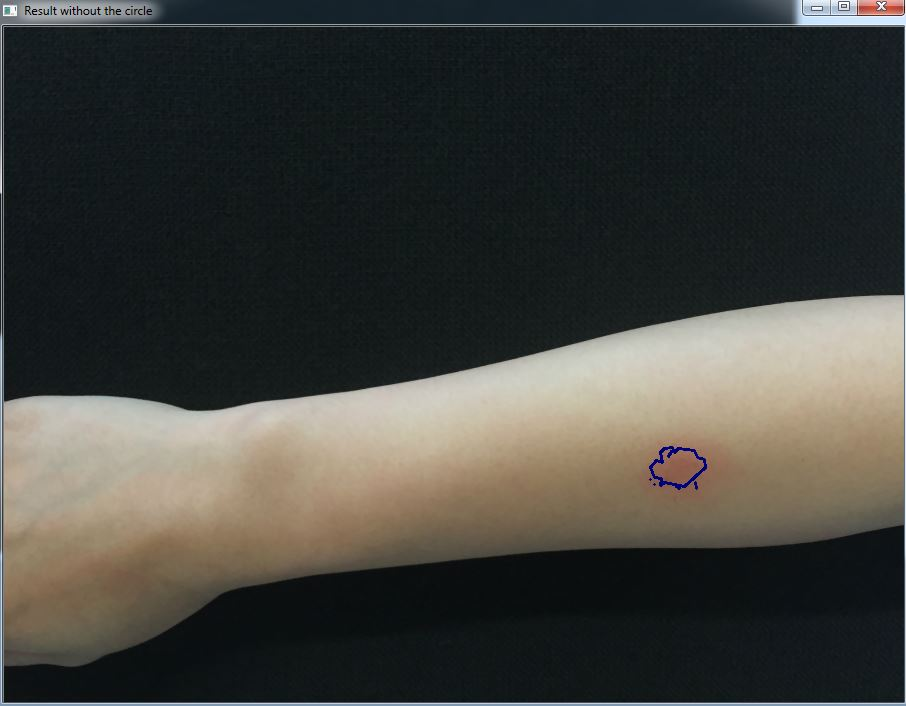
\includegraphics[width=8cm,height=6cm]{img/detectresult0circle}
  \caption{Draw contours polygons Image1 with s(100, 255)\cite{Bradski}}
  \label{fig:sub1}
\end{subfigure}%
\begin{subfigure}{.5\textwidth}
  \centering
  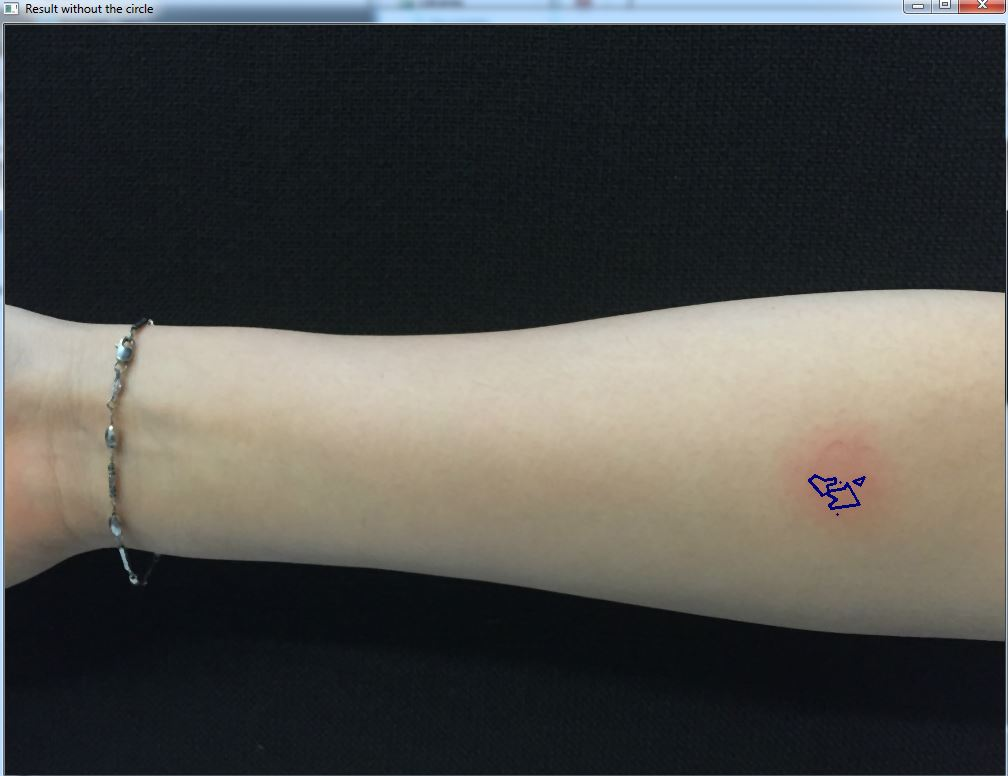
\includegraphics[width=8cm,height=6cm]{img/detectresult0circle2}
  \caption{Draw contours polygons Image2 with s(100, 255)}
  \label{fig:sub2}
\end{subfigure}
\caption{Draw contours polygons Image with s(100, 255)}
\label{fig:test}
\end{figure}

 \begin{figure}[!h]
\centering
\begin{subfigure}{.5\textwidth}
  \centering
  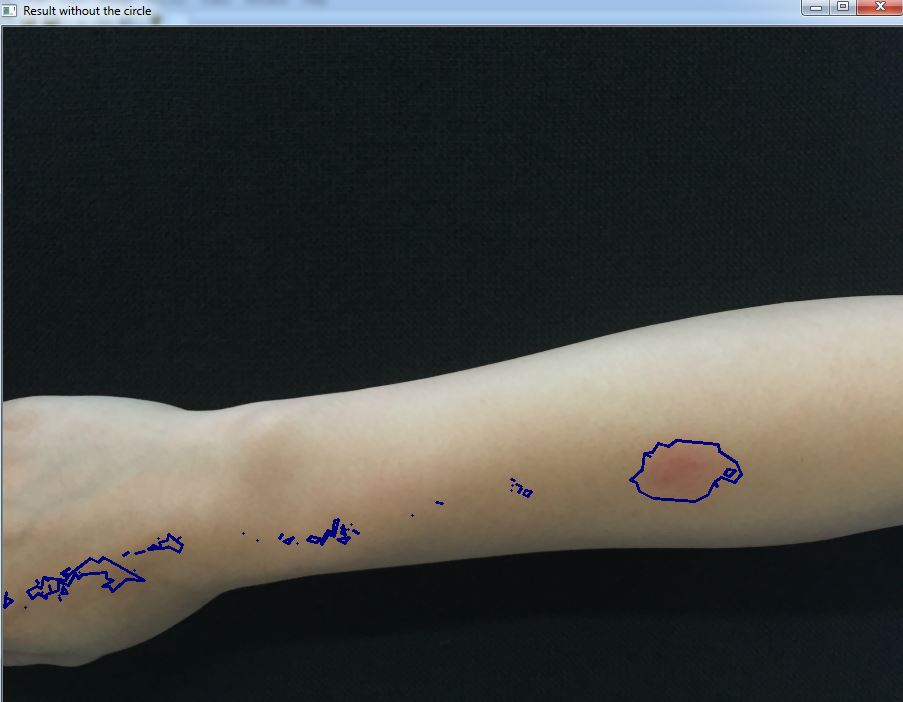
\includegraphics[width=8cm,height=6cm]{img/4}
  \caption{Draw contours polygons Image1 with s(95, 255)}
  \label{fig:sub1}
\end{subfigure}%
\begin{subfigure}{.5\textwidth}
  \centering
  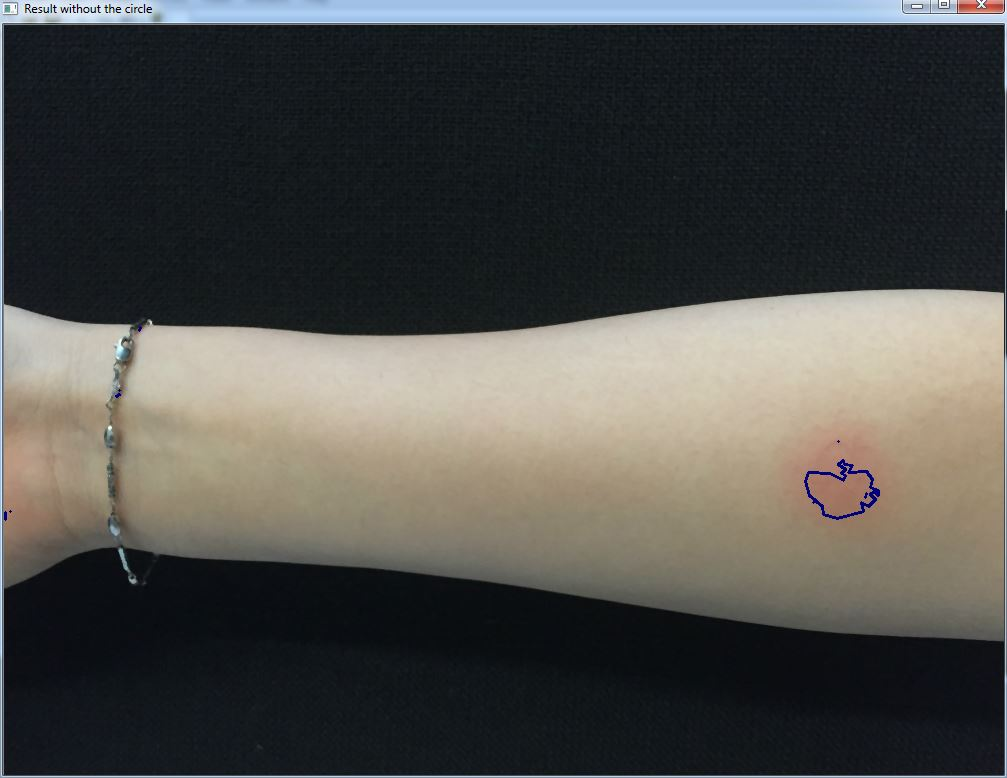
\includegraphics[width=8cm,height=6cm]{img/2}
  \caption{Draw contours polygons Image2 with s(95, 255)}
  \label{fig:sub2}
\end{subfigure}
\caption{Draw contours polygons Image with s(95, 255)}
\label{fig:test}
\end{figure}


 \begin{figure}[!h]
\centering
\begin{subfigure}{.5\textwidth}
  \centering
  \includegraphics[width=8cm,height=6cm]{img/detectresult1circle}
  \caption{Draw contours polygons with circle Image1}
  \label{fig:sub1}
\end{subfigure}%
\begin{subfigure}{.5\textwidth}
  \centering
  \includegraphics[width=8cm,height=6cm]{img/detectresult1circle2}
  \caption{Draw contours polygons with circle Image2}
  \label{fig:sub2}
\end{subfigure}
\caption{Draw contours polygons with circle Image}
\label{fig:test}
\end{figure}

\newpage
\section{Eulerian Color Magnification}
The human visual system has limited spatio-temporal sensitivity, but many signals that fall below this capacity can be informative.  This variation, while invisible to the naked eye, can be exploited to extract pulse rate \cite{Verkruysse} \cite{Poh}. This section shows that a combination of temporal and spatial processing of videos can amplify subtle color variations.\\

Eulerian Video Magnification \cite{Rubinstein} considers the time series of color values at every spatial pixel and reveal the signal corresponding to the cardiac pulse. It allows to amplify variations in a given temporal frequency band of interest. This method creates potential for diagnostic and monitoring applications to medicine, such as the asymmetry in facial blood flow maybe a symptom of arterial problems.\\

This method illustrated in Figure 5.24, Combines spatial and temporal processing to large the subtle temporal changes in the video. Firstly, the video sequence is decomposed into different spatial frequency bands because they might exhibit different signal-to-noise ratios and be magnified differently. Secondly, use temporal processing on each spatial band. The temporal processing is uniform for all the spatial bands, and for all pixels within each band. Thirdly, the extracted
bandpass signal is magnified by the  amplification Factor. Finally, the magnified signal is added to the original image and the
spatial pyramid collapsed to obtain the final output. Details are discribed in the next section.\\
\begin{figure}[!htb]
	\centering
	\includegraphics[scale=0.55]{img/processdiagram}
	\caption{Eulerian Color Magnification Process Diagram}
\end{figure}


\subsection{Spatial Decomposition}
For extracting required information from an image, it is necessary to be passed through a combination of different filters, with different sequences depending on
the requirements.\\

The visual sense of human beings is very intuitive. It has the properties
of less spatio-temporal sensitivity. The detection of variations on color at lower spatial amplitudes is almost impossible for the human sense of vision. Image pyramid is used to reveal subtle changes in videos. A pyramid is developed by computer vision, image and signal processing fields. It is applied for signal representation at multiple scales. So the first step is to compute a layer of the Gaussian pyramid, which may be obtained by successively scaling down the image by calculating the Gaussian average for each pixel.\\

Gaussian pyramid \cite{Aurich} is used in forming large scale digital images mathematically and graphically using different algorithms from small digital samples of an image.  Consider that the bottom level of the Pyramid G0 is equivalent to the original image. Figure is subsampled by a factor of 4 and low pass filtered to from the next level of the pyramid G1. Repeat the process in order
to get to the next level in the pyramid. This can be represented in terms of
equation from $0 < 1 < N$ : 
\begin{displaymath}
G\left ( i,j \right ) \sum_{m} \sum_{n} w\left ( m,n \right )G_{j}-1\left ( 2i+m,2j+n \right )
\end{displaymath}

The $w\left ( m,n \right )$ needs function named as generating kernel using the small and sparable $w\left ( m,n \right )$ to obtain the promising efficiency. The pyramid contrastion is considered as equivalent to convolving the original image with the set of Gaussian and at every level of pyramid, the function width always increase to double. It is also considered as that it acts as a low pass filter.\\

In this report, using opencv pyrDown() function, by default, size of the output image is computed as Size((src.cols+1)/2, (src.rows+1)/2), but in any case, the following conditions should be satisfied:
\begin{displaymath}
\left | dstsize.with*2-src.cols \right | < 2 
\end{displaymath}
\begin{displaymath}
\left | dstsize.height*2-src.rows \right | < 2 
\end{displaymath}
And the function performs the downsampling step of the Gaussian pyramid construction. Figure 5.25 shows the example. 
 \begin{figure}[!h]
\centering
\begin{subfigure}{.6\textwidth}
  \centering
  \includegraphics[scale=0.16]{img/eulerian/sample/test}
  \caption{Original}
  \label{fig:sub1}
\end{subfigure}%
\begin{subfigure}{.6\textwidth}
  \centering
  \includegraphics[scale=0.16]{img/eulerian/sample/0}
  \caption{G1}
  \label{fig:sub2}
\end{subfigure}
\begin{subfigure}{.3\textwidth}
  \centering
  \includegraphics[scale=0.16]{img/eulerian/sample/1}
  \caption{G2}
  \label{fig:sub2}
\end{subfigure}
\begin{subfigure}{.3\textwidth}
  \centering
  \includegraphics[scale=0.16]{img/eulerian/sample/2}
  \caption{G3}
  \label{fig:sub2}
\end{subfigure}
\begin{subfigure}{.3\textwidth}
  \centering
  \includegraphics[scale=0.16]{img/eulerian/sample/3}
  \caption{G4}
  \label{fig:sub2}
\end{subfigure}
\caption{Gaussian Pyramid}
\label{fig:test}
\end{figure}

In terms of the sample density those levels are not the same. Therefore, it is important that these new levels should be interpolated
between those at a given level and after that level it is subtracted from the next level which is low. This whole process could be formed by reversing the REDUCE process and so called EXPAND process. Figure 5.26 presents level of the Gaussian pyramid expanded to size of original image.\\
 \begin{figure}[!h]
\centering
\begin{subfigure}{.5\textwidth}
  \centering
  \includegraphics[width=7.5cm,height=4.5cm]{img/eulerian/sample/test}
  \caption{Original}
  \label{fig:sub1}
\end{subfigure}%
\begin{subfigure}{.5\textwidth}
  \centering
  \includegraphics[width=7.5cm,height=4.5cm]{img/eulerian/sample/0}
  \caption{G1}
  \label{fig:sub2}
\end{subfigure}
\begin{subfigure}{.5\textwidth}
  \centering
  \includegraphics[width=7.5cm,height=4.5cm]{img/eulerian/sample/1}
  \caption{G2}
  \label{fig:sub2}
\end{subfigure}%
\begin{subfigure}{.5\textwidth}
  \centering
  \includegraphics[width=7.5cm,height=4.5cm]{img/eulerian/sample/2}
  \caption{G3}
  \label{fig:sub2}
\end{subfigure}
\caption{Level of the Gaussian pyramid expanded to size of original image}
\label{fig:test}
\end{figure}

\newpage
If $G_{l,k}$ is the image obtained by expanding $G_{l}$ k times. Then $G_{l,k}=EXPAND\left [ GG_{l,k-1} \right ]$, or to be precise $G10=G_{l,0}=G_{l}$, for $k>0$,

\begin{displaymath}
G_{i,j}\left (i.j \right )=4 \sum_{m}\sum_{n}G_{l,k-1}\left ( \frac{2i+m}{2},\frac{2j+n}{2} \right )
\end{displaymath}

$(2i + m)=2$ and $(2j + n)=2$ are integers contribute to
the sum. In the case of the expand operation, double the size of the image with each iteration, so that $G_{l,1}$ is the size and  $G_{l,1}$ same size as that of the original image. \\

Band pass level or the Pyramid $L_{0}, L_{1},,...,L_{N}$ may be specified in terms of low pass pyramid level as below.
\begin{displaymath}
L_{l}=G-EXPAND\left [ l+1 \right ]
\end{displaymath}
\begin{displaymath}
L_{l}=G_{1}-G_{l+1,1}
\end{displaymath}
The value at each node in Gaussian Pyramid can be obtained by convolving a Gaussian like equivalent weighting function with the original image.

\subsection{Temporal Filtering}
Before go to the next step, concat all the frames into a single large Mat where each column is a reshaped single frame, this is for processing convenience.
 \begin{figure}[!h]
\centering
\begin{subfigure}{.6\textwidth}
  \centering
  \includegraphics[scale=0.18]{img/eulerian/sample/test}
  \caption{Original Hand Video Frame}
  \label{fig:sub1}
\end{subfigure}%
\begin{subfigure}{.5\textwidth}
  \centering
  \includegraphics[scale=0.1]{img/eulerian/sample/ress}
  \caption{Cancat all the frames}
  \label{fig:sub2}
\end{subfigure}
\begin{subfigure}{.45\textwidth}
  \centering
  \includegraphics[scale=0.4]{img/eulerian/sample/orginalRGB}
  \caption{RGB diagram of image after gaussian pyramid}
  \label{fig:sub2}
\end{subfigure}
\begin{subfigure}{.45\textwidth}
  \centering
  \includegraphics[scale=0.4]{img/eulerian/sample/nextRGB}
  \caption{RGB diagram of concatenate image after gaussian pyramid}
  \label{fig:sub2}
\end{subfigure}
\caption{Frams(image) after gaussian pyramid}
\label{fig:test}
\end{figure}

\newpage
Temporal filtering is used to extract the signals to be amplified. Thus, the filter choice is application dependent. Figure 5.24 shows frequency responses of some of the temporal filters used in the present paper. For motion magnification, a broad bandpass filter is preferred.For a real-time implementation low-order IIR filters can be useful for color amplification. And an ideal bandpass filter is used on due to its sharp cutoff. The temporal processing is uniform for all the spatial levels, and for all the pixels within each level \cite{Rubinstein}. This report used ideal temporal filters. \\

\begin{figure}[!htb]
	\centering
	\includegraphics[scale=0.55]{img/eulerian/temperial}
	\caption{Examples of temporal filters:  (a) and (b) show ideal filters with sharp cut off frequencies, (c) shows a so called Butterworth filter, that has as flat a frequency response as possible in the passband [13] and (d) shows a so called second-order IIR filter with a broad frequency passband. Under each image there is a note in brackets that specifies on which video was each filter used. (source: \cite{Christiano})}
\end{figure}

\newpage
Ideal Band pass Filter \cite{Christiano} was used for color amplification because it has sharp cut off frequencies. The signal of color changes is kind of weak. An ideal band pass filter is defined as the one that allows frequencies to pass if they are between two specified frequencies, which is $(f_{l}, f_{h})$. Filter circuits can be designed to accomplish the task by combining the properties of low-pass and high-pass into one single filter. Creating a bandpass filter from a low-pass and high-pass filter can be illustrated using block diagrams: \\

\begin{figure}[!htb]
	\centering
	\includegraphics[scale=0.55]{img/idealband}
	\caption{System level block diagram of a band-pass filter}
\end{figure}

What's more, ideal band pass filter requires: between two specified frequencies, frequency response $H\left ( e^{j2\pi fTs } \right )=1$, while out of the range $H\left ( e^{j2\pi fTs } \right )=0$. So $H(f)$ is defined as:
\[
    H(f)=\left\{
                \begin{array}{ll}
                  1 & f_{l} <|f|<  f_{h}\\
                  0 & otherwise\\
                \end{array}
              \right.
\]
  
$f_{l}$ is the low-pass frequency and $f_{h}$ is the high-pass frequency. The amplitude spectrum is shown in Figure 5.25.
\begin{figure}[!htb]
	\centering
	\includegraphics[scale=0.6]{img/idealband2}
	\caption{The amplitude spectrum for the ideal band pass filter}
\end{figure}
Based on the report, face color magnification uses the frequency from 0.8Hz to 1Hz.\\

\newpage
For color amplification, it test samples (Figure 5.30) with different skin colors and different positions. One with dark complexity another one with a light skin color, in order to observe changes in their skin color as blood flows through the faces.\\

 \begin{figure}[!h]
\centering
\begin{subfigure}{.5\textwidth}
  \centering
  \includegraphics[scale=0.25]{img/eulerian/test/man}
  \caption{Face Sample 1}
  \label{fig:sub1}
\end{subfigure}%
\begin{subfigure}{.5\textwidth}
  \centering
  \includegraphics[scale=0.35]{img/eulerian/test/man2}
  \caption{Face Sample 2}
  \label{fig:sub2}
\end{subfigure}
\begin{subfigure}{.5\textwidth}
  \centering
  \includegraphics[width=7.5cm]{img/eulerian/test/hand}
  \caption{Hand Sample 1}
  \label{fig:sub1}
\end{subfigure}%
\begin{subfigure}{.5\textwidth}
  \centering
  \includegraphics[width=7.5cm]{img/eulerian/test/hand2}
  \caption{Hand Sample 2}
  \label{fig:sub2}
\end{subfigure}
\begin{subfigure}{.5\textwidth}
  \centering
  \includegraphics[width=7.5cm]{img/eulerian/test/leg}
  \caption{Leg Sample 1}
  \label{fig:sub1}
\end{subfigure}%
\begin{subfigure}{.5\textwidth}
  \centering
  \includegraphics[width=7.5cm]{img/eulerian/test/leg2}
  \caption{Leg Sample 1}
  \label{fig:sub2}
\end{subfigure}
\caption{Videos used for experiment}
\label{fig:test}
\end{figure}
How to achieve temporal filtering in OpenCV? Follow the steps below, note that here the cancated image is on the process, rather the original one for calculation convenience:
\begin{enumerate}
    \item Split the image into three channels to deal with every channel
    \item Make the Discrete Fourier Transform (DFT). The performance of a DFT depends on the image size. It is fastest for image sizes that are multiple of the numbers 2, 3 and 5. Therefore, to achieve maximal performance, pad border values to the image to get a size with such traits.
    \item Construct the filter (Ideal Band pass Filter). Only allows frequencies to pass if they are between $f_{l},f{_h}$, set value 1, otherwise the value is 0.
    \item Apply the filter. Simple multiple with an optional conjugation, which is the result of previous step obtains.
    \item Do the inverse DFT on the filtered image. Calculates the inverse Discrete Fourier Transform of a 1D or 2D array.
    \item Copy back to the current channel.
    \item Merge three channels.
    \item Normalize the filtered image, since the image display range of zero to one.
\end{enumerate}

The Fourier Transform \cite{Bracewell} decomposes an image into its sinus and cosines components. That means, it transforms an image from its spatial domain to its frequency domain. Mathematically, the two dimensional images Fourier transform is defined as:
\begin{displaymath}
F\left ( k,l \right )=\sum_{i=0}^{N-1}\sum_{j=0}^{N-1}f\left ( i,j \right )e^{-i2\pi \left ( \frac{ki}{N}+ \frac{lj}{N} \right )}
\end{displaymath}
\begin{displaymath}
e^{ix}=cos\left ( x \right )+isin\left ( x \right )
\end{displaymath}

$f$ is the image value in its spatial domain and $F$ is that in its frequency domain. The result of the transformation is complex numbers. Displaying this is either via a real image and a complex image or via a magnitude and a phase image. However, only the magnitude image contains all the information needed about the images geometric structure. If you intend to make some modifications of the image in these forms, it is important to retransform it and preserve both.\\



\subsection{Amplification Factor}
After extracting the required band of frequencies which is going to be amplified like color, those bands are exaggerated by a factor alpha. To amplify is straight forward, for color magnification, artifacts is acceptable, just amplify the selected frequency from the top of the pyramid at a constant rate. These values can be controlled by the user depending upon application requirements. Best value or an optimized value can be obtained by doing experimentation and observing results. There is a risk that noise could increase. If it is needed to amplify a human color, an emphasis should be laid on lower spatial frequencies. \\

After amplification, adding frame image and the result image to get magnified image and write into video. Figure shows how do ideal band pass filter and amplication works.\\

Various combinations of $\alpha$ and $\lambda_{c}$ can be used, also those that violate the bounds to exaggerate the specific color changes at the cost of increasing noise or introducing more artifacts. The details will discribe in the Chapter 6.\\


 \begin{figure}[!h]
\centering
\begin{subfigure}{.23\textwidth}
  \centering
  \includegraphics[scale=0.1]{img/eulerian/sample/tempp}
  \caption{concatenate image}
  \label{fig:sub2}
\end{subfigure}
\begin{subfigure}{.23\textwidth}
  \centering
  \includegraphics[scale=0.2]{img/eulerian/test/temp}
  \caption{concatenate image}
  \label{fig:sub2}
\end{subfigure}
\begin{subfigure}{.5\textwidth}
  \centering
  \includegraphics[scale=0.5]{img/eulerian/sample/filterRGB}
  \caption{RGB Histogram of filtered image}
  \label{fig:sub2}
\end{subfigure}
\caption{Frams(image) after ideal band pass filter}
\label{fig:test}
\end{figure}
The following figures show how temporal ideal bandpass and filter and amplification work step by step. Figure 5.32 shows temporal ideal bandpass filtering result. The right one is RGB histogram of the filtered image. Figure 5.33 shows the result after amplification. Add the filtered image to the original image, then get Figure 5.34 and Figure 5.35.\\

 \begin{figure}[!h]
\centering
\begin{subfigure}{.4\textwidth}
  \centering
  \includegraphics[scale=0.1]{img/eulerian/sample/tempp2}
  \caption{amplify concatenate filtered image}
  \label{fig:sub1}
\end{subfigure}%
\begin{subfigure}{.5\textwidth}
  \centering
  \includegraphics[scale=0.5]{img/eulerian/sample/amplifyRGB}
  \caption{RGB diagram of filtered image after amplification}
  \label{fig:sub2}
\end{subfigure}
\caption{Frams(image) after amplification}
\label{fig:test}
\end{figure}

\begin{figure}[!h]
	\centering
	\includegraphics[scale=0.2]{img/eulerian/sample/30}
	\caption{Original image added magnificant image in 1 second}
\end{figure}
\begin{figure}[!h]
	\centering
	\includegraphics[scale=0.2]{img/eulerian/sample/120}
	\caption{Original image added magnificant image in 3 second}
\end{figure}
\newpage
Figure 5.34 and 5.35  shows screenshots of video taken after the color magnification procedure on arm. More reddish areas mean greater
amplitude of blood volume pulse in hands. Local red area input affects the vascular system and this cause blood perfusion changes. There is clearly seen that
amplitude of blood pulsations increases 2 minute. Increasing of blood flow means increasing of haemoglobin concentration on subcutaneous tissue. \\

Figure 5.36 shows the dynamics of B and G signals from normal skins area and pressure ulceres area forearm
skin. Because microcirculation B and G signals are inverse-proportional to redness of skin, increasing of blood microcirculation cause decreasing of amplitudes of B and G signals. 
 \begin{figure}[!h]
\centering
\begin{subfigure}{.5\textwidth}
  \centering
  \includegraphics[scale=0.25]{img/noisepos}
  \caption{Red point in the original frames}
  \label{fig:sub1}
\end{subfigure}%
\begin{subfigure}{.5\textwidth}
  \centering
  \includegraphics[scale=0.25]{img/change}
  \caption{The dynamics of B and G signals changes}
  \label{fig:sub2}
\end{subfigure}
\caption{The dynamics of B and G signals changes of the red point in the left figure}
\label{fig:test}
\end{figure}

\newpage
\section{Other Edit Functions}
\subsection{Rotation}
Rotation operator performs a geometric transform which maps the position $(x_{1},y_{1})$ of a picture element in an input image onto a position $(x_{2},y_{2})$ in an output image by rotating it through the specified angle $\theta$  about an origin. In most implementations, output locations $(x_{2},y_{2})$, which are outside the boundary of the image are ignored. Rotation is commonly used to improve the visual appearance of an image, although it can be useful as a preprocessor in applications where directional operators are involved. Rotation is the special case of affine transformation.\\

The rotation operator performs a transformation of the form:
\begin{displaymath}
x_{2}=cos\left ( \theta  \right )\left ( x_{1}-x_{0} \right )-sin\left ( \theta  \right )\left ( y_{1}-y_{0} \right )+x_{0}
\end{displaymath}
\begin{displaymath}
y_{2}=sin\left ( \theta  \right )\left ( x_{1}-x_{0} \right )-cos\left ( \theta  \right )\left ( y_{1}-y_{0} \right )+y_{0}
\end{displaymath}
$(x_{0},y_{0})$ is the coordinates of the center of rotation of the input image, $\theta$ is the angle of rotation with the clockwise rotations having positive angles. Even more than the translate operator, the rotation operation produces output locations $(x_{1},y_{1})$ which do not fit within the boundaries of the image. In such cases, destination elements which are mapped outside the image are ignored by most implementations. Pixel locations out of which an image has been rotated are usually filled in with black pixels.\\

\subsection{Scaling}
Scaling operator performs the geometric transformation, which can be used to zoom the size of an image. Image reduction, is ahieved by replacement of a group of pixel values by the one arbitrarily chosen pixel value from this group, or by interpolating between pixel values in the local neighborhoods. Image zooming is performed by pixel replication or interpolation. Scaling is used to change the visual appearance of an image, to alter the quantity of information stored in a scene representation, or as a low-level preprocessor in multiple stage image processing chain, which operates on features of a particular scale. \\

Scaling expands or compresses an image along the coordinate directions. Figure 5.36 presents the two methods of sub-sampling. Left one is, one pixel value within a local neighborhood is chosen, to be representative of its surroundings. This method is computationally simple, but may lead to poor results if the sampling neighborhoods are too large. The right method is to, interpolate between pixel values within a neighborhood by taking a statistical sample (i.e. the mean) of the local intensity values.
\begin{figure}[!h]
	\centering
	\includegraphics[scale=0.75]{img/method}
	\caption{Methods of subsampling: Replacement with upper left pixel and Interpolation using the mean value}
\end{figure}

\newpage
An image can be zoomed either through interpolation or  pixel replication. Figure 5.37 shows how pixel replication simply replaces each original image pixel by the group of pixels with the same value, where the group size is determined by the scaling factor. Alternatively, interpolation of the values of neighboring pixels in the original image can be performed in order to replace each pixel with an expanded group of pixels. 

\begin{figure}[!h]
	\centering
	\includegraphics[scale=0.75]{img/method2}
	\caption{Methods of zooming: Replication of a single pixel value and Interpolation}
\end{figure}